%% ------------------------------------------------------------------------- %%
\chapter{Moda das Ondas no Tower Defense para versão v1}
\label{sec:apend-moda-td-v1}

Foram calculadas as modas das ondas do \textit{fitness} desenvolvido, para permitir a visualização dos inimigos mais comuns que o algoritmo convergiu.

%% ------------------------------------------------------------------------- %%
\section{Torres Verdes}
\label{sec:apend-moda-td-g-v1}

\begin{figure}[H]
  \centering
  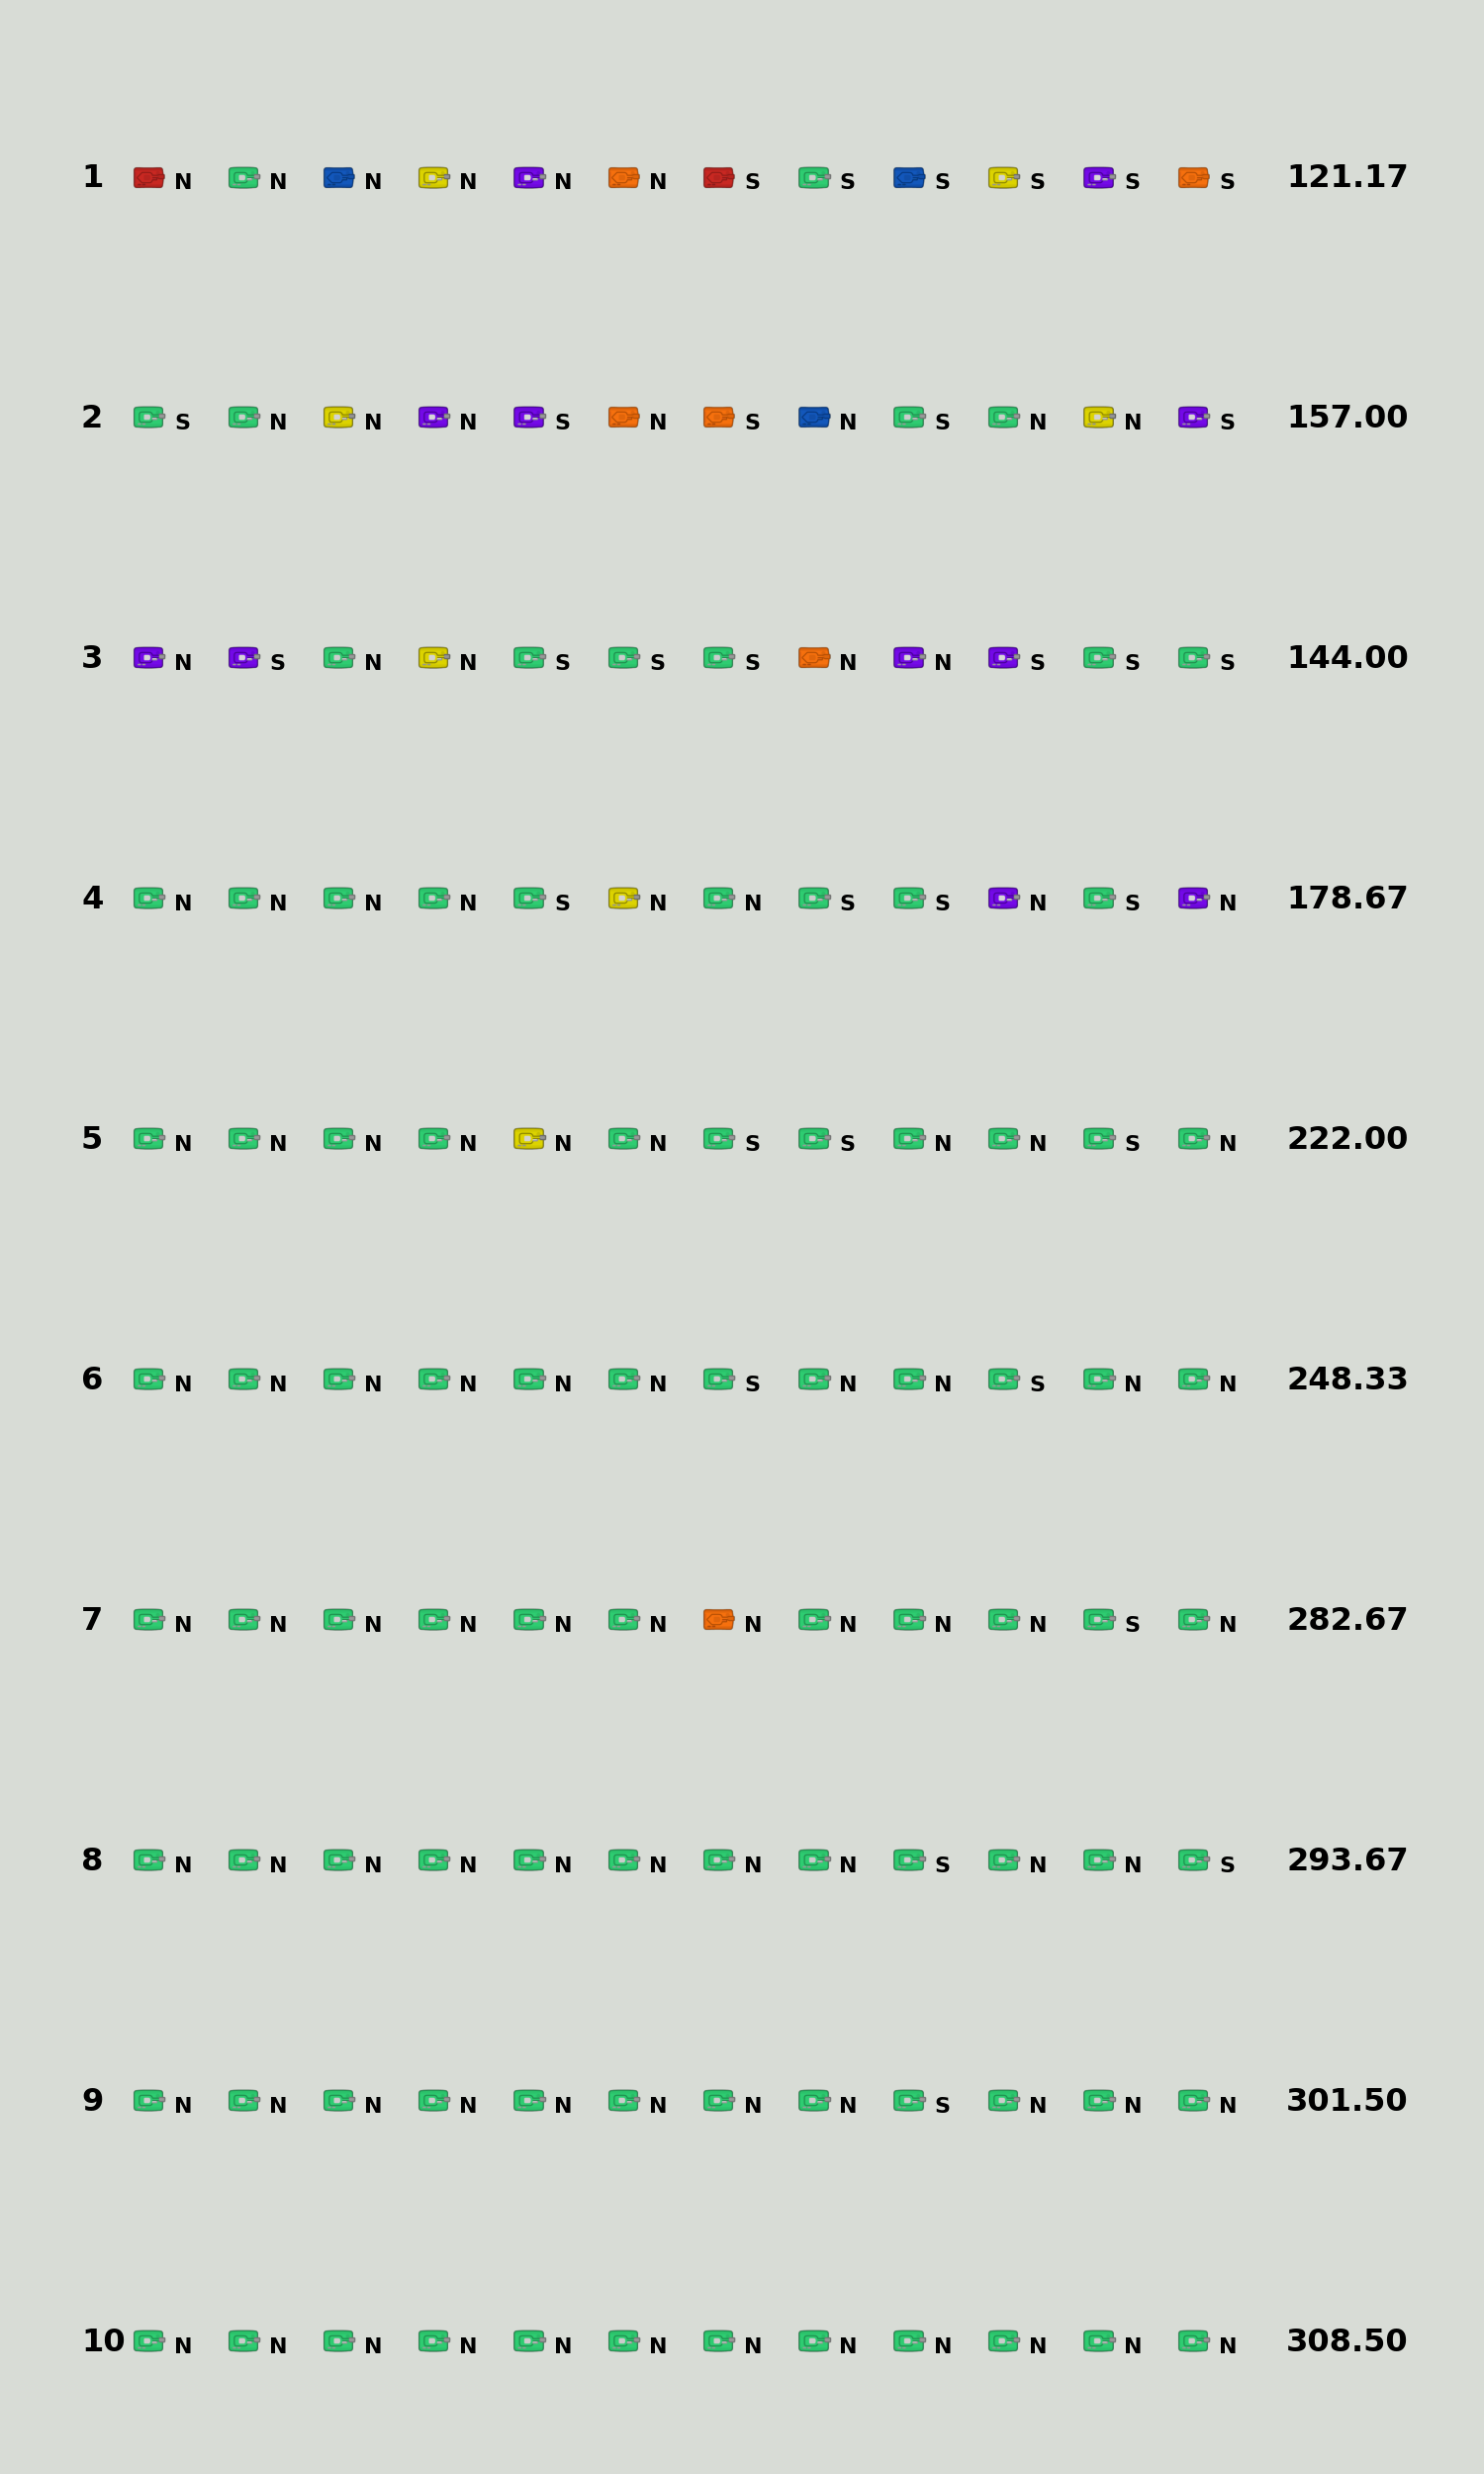
\includegraphics[width=0.9\textwidth]{figuras/td/td_allgreen_ai_mode_1_1.png}
  \caption{Visualização da moda de cada onda com a versão v1 contra Torres Verdes.}
  \label{fig:td-moda-green-1-1}
\end{figure}

\begin{figure}[H]
  \centering
  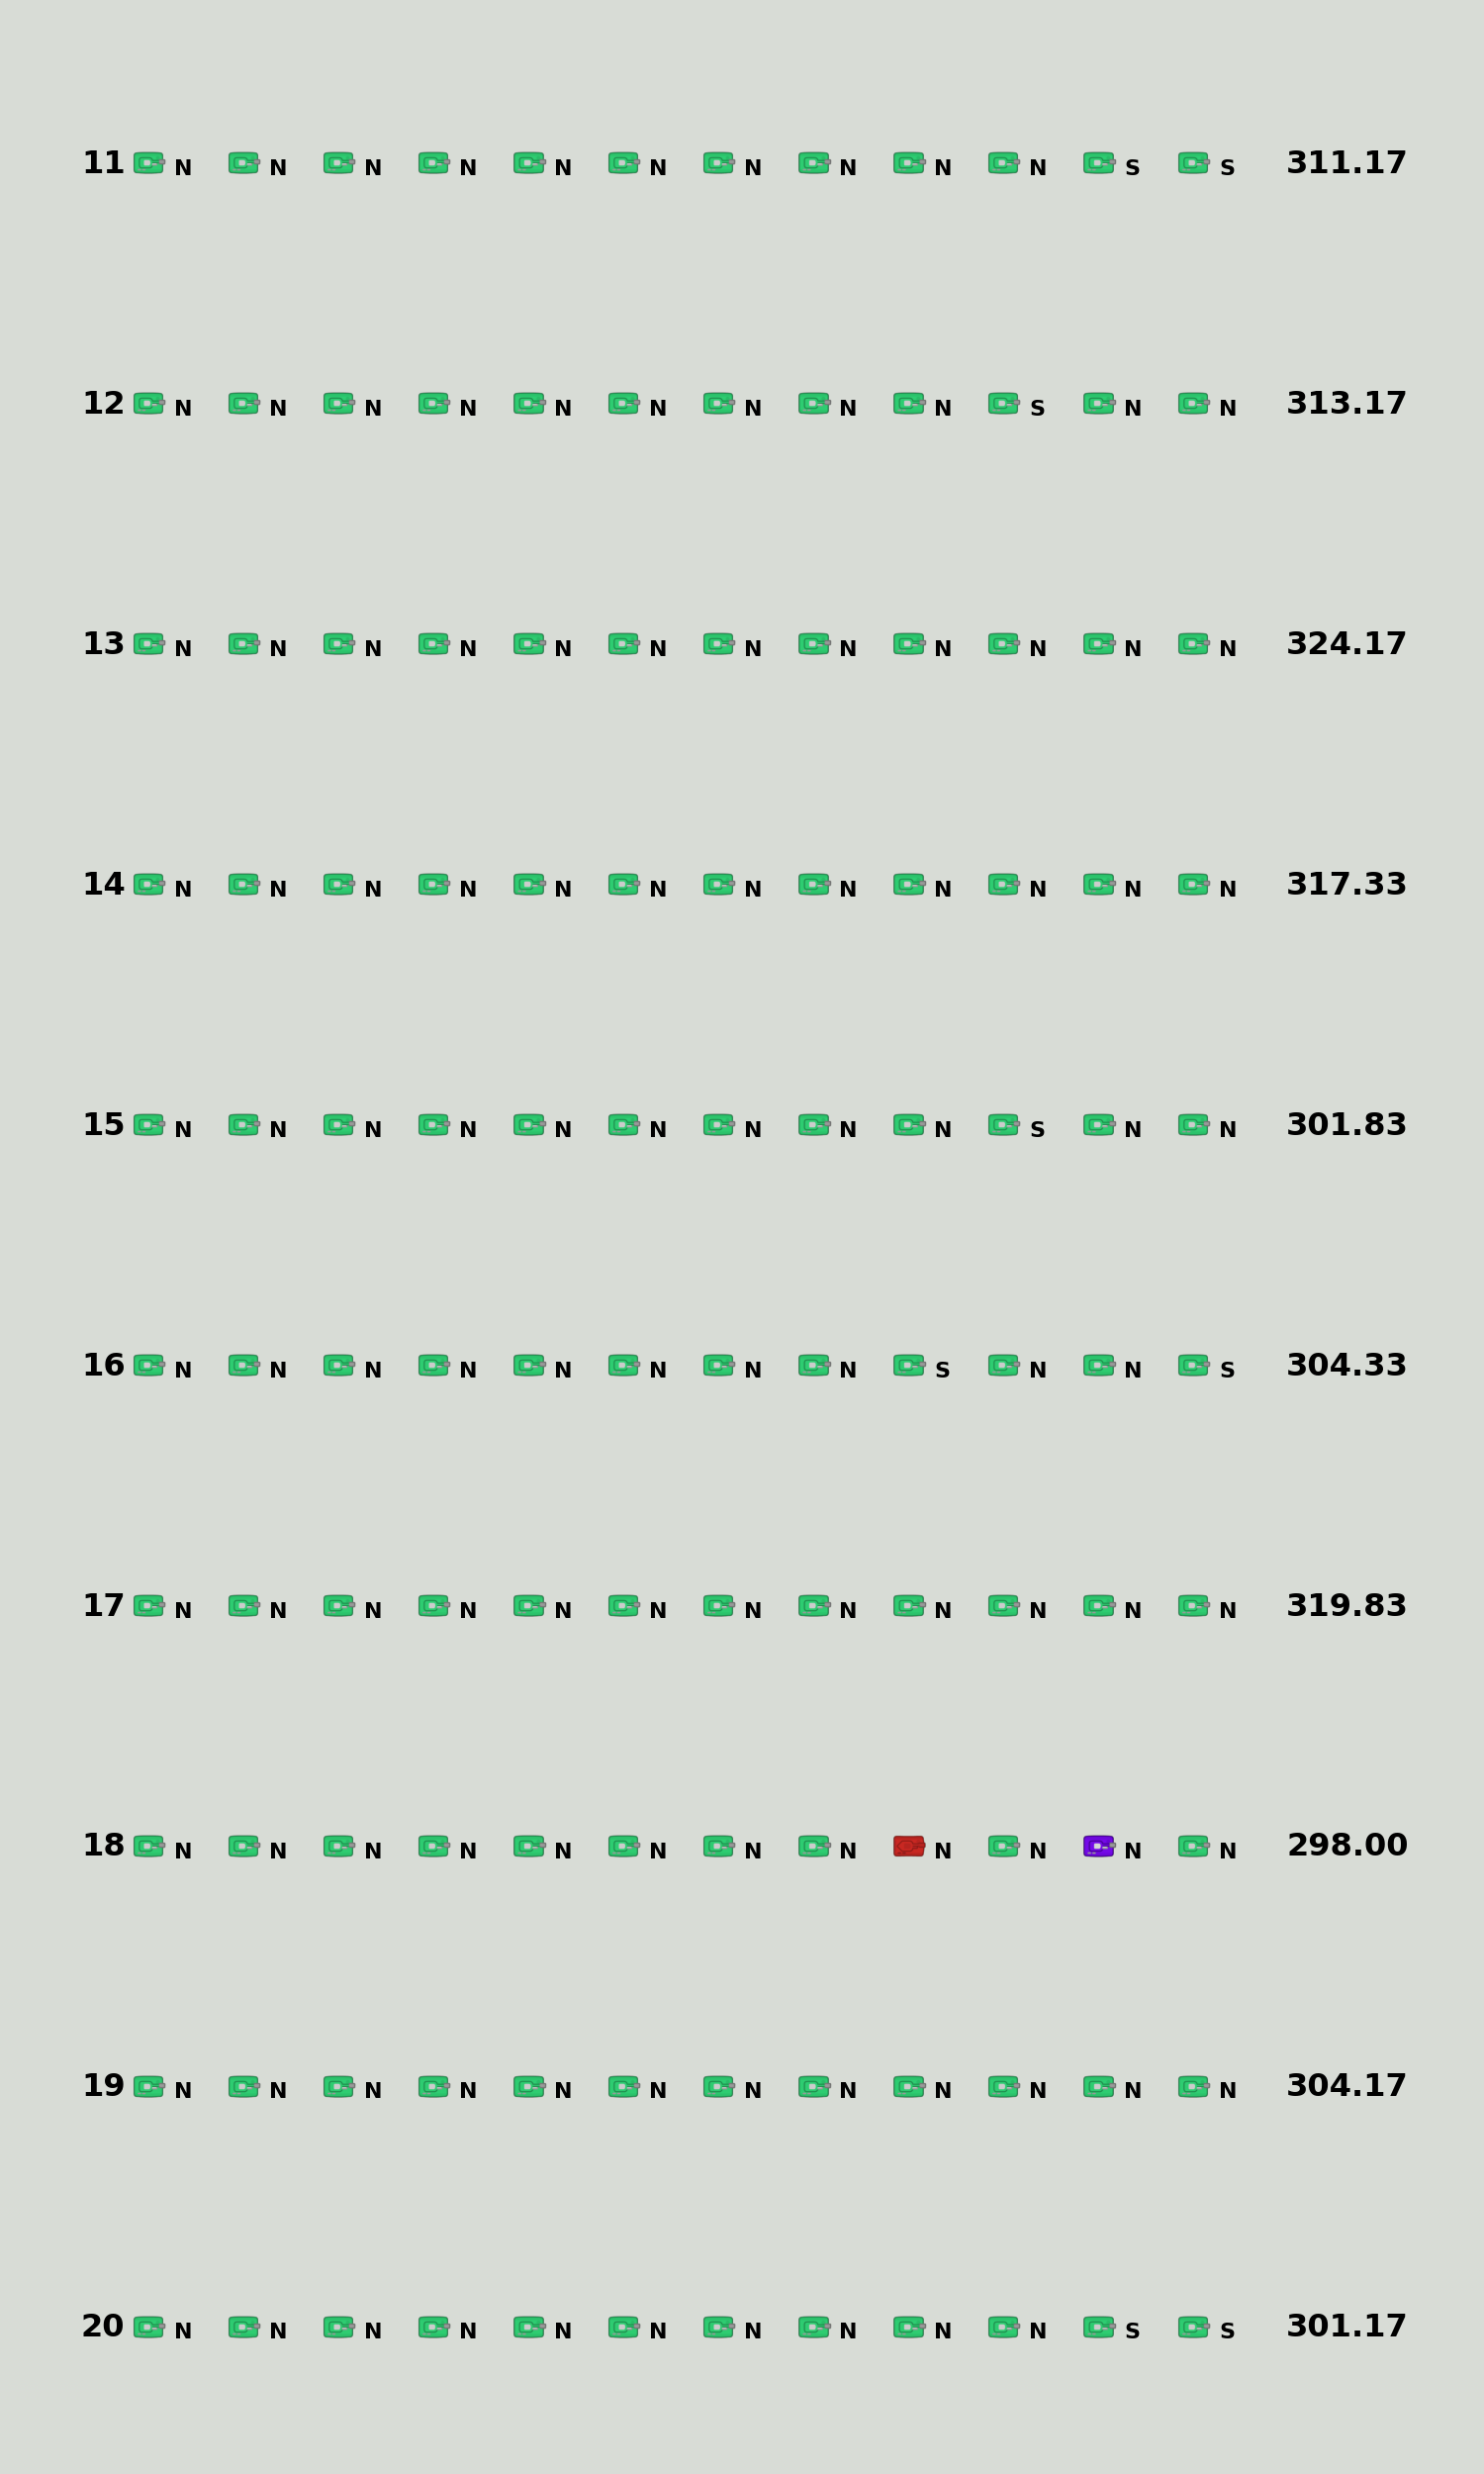
\includegraphics[width=0.9\textwidth]{figuras/td/td_allgreen_ai_mode_1_2.png}
  \caption{Visualização da moda de cada onda com a versão v1 contra Torres Verdes.}
  \label{fig:td-moda-green-1-2}
\end{figure}

\begin{figure}[H]
  \centering
  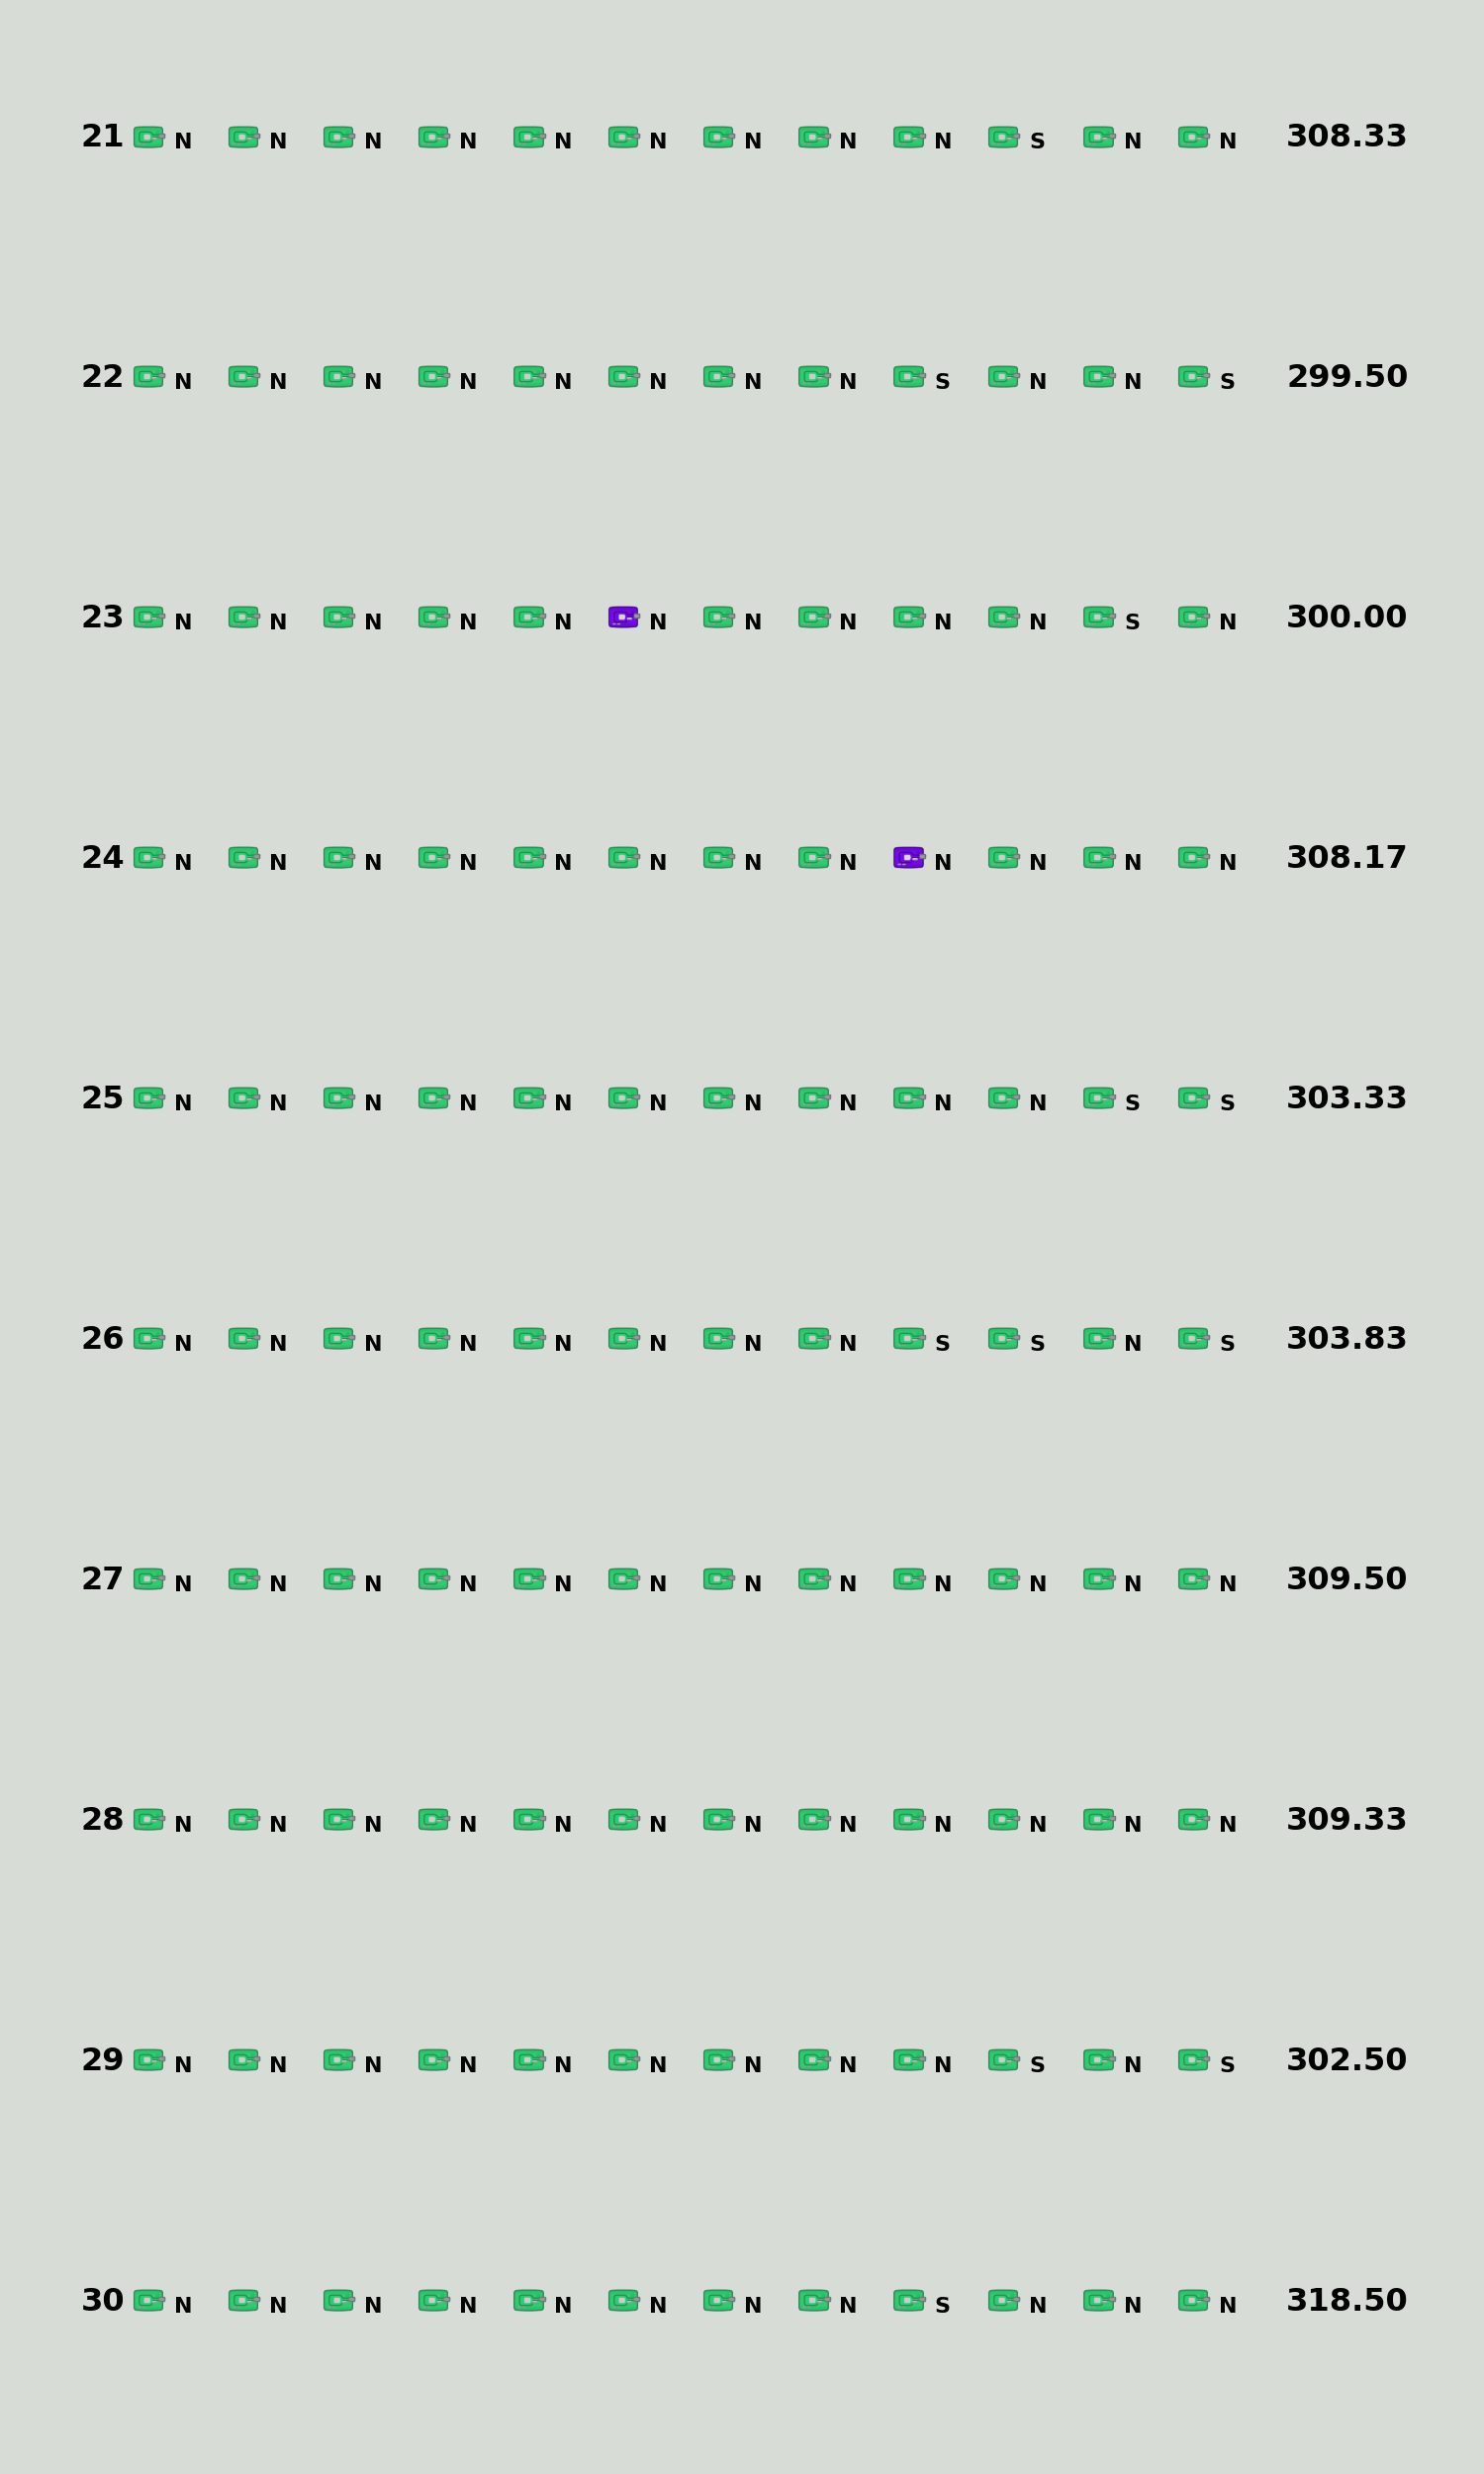
\includegraphics[width=0.9\textwidth]{figuras/td/td_allgreen_ai_mode_1_3.png}
  \caption{Visualização da moda de cada onda com a versão v1 contra Torres Verdes.}
  \label{fig:td-moda-green-1-3}
\end{figure}

%% ------------------------------------------------------------------------- %%
\section{Torres Vermelhas}
\label{sec:apend-moda-td-r-v1}

\begin{figure}[H]
  \centering
  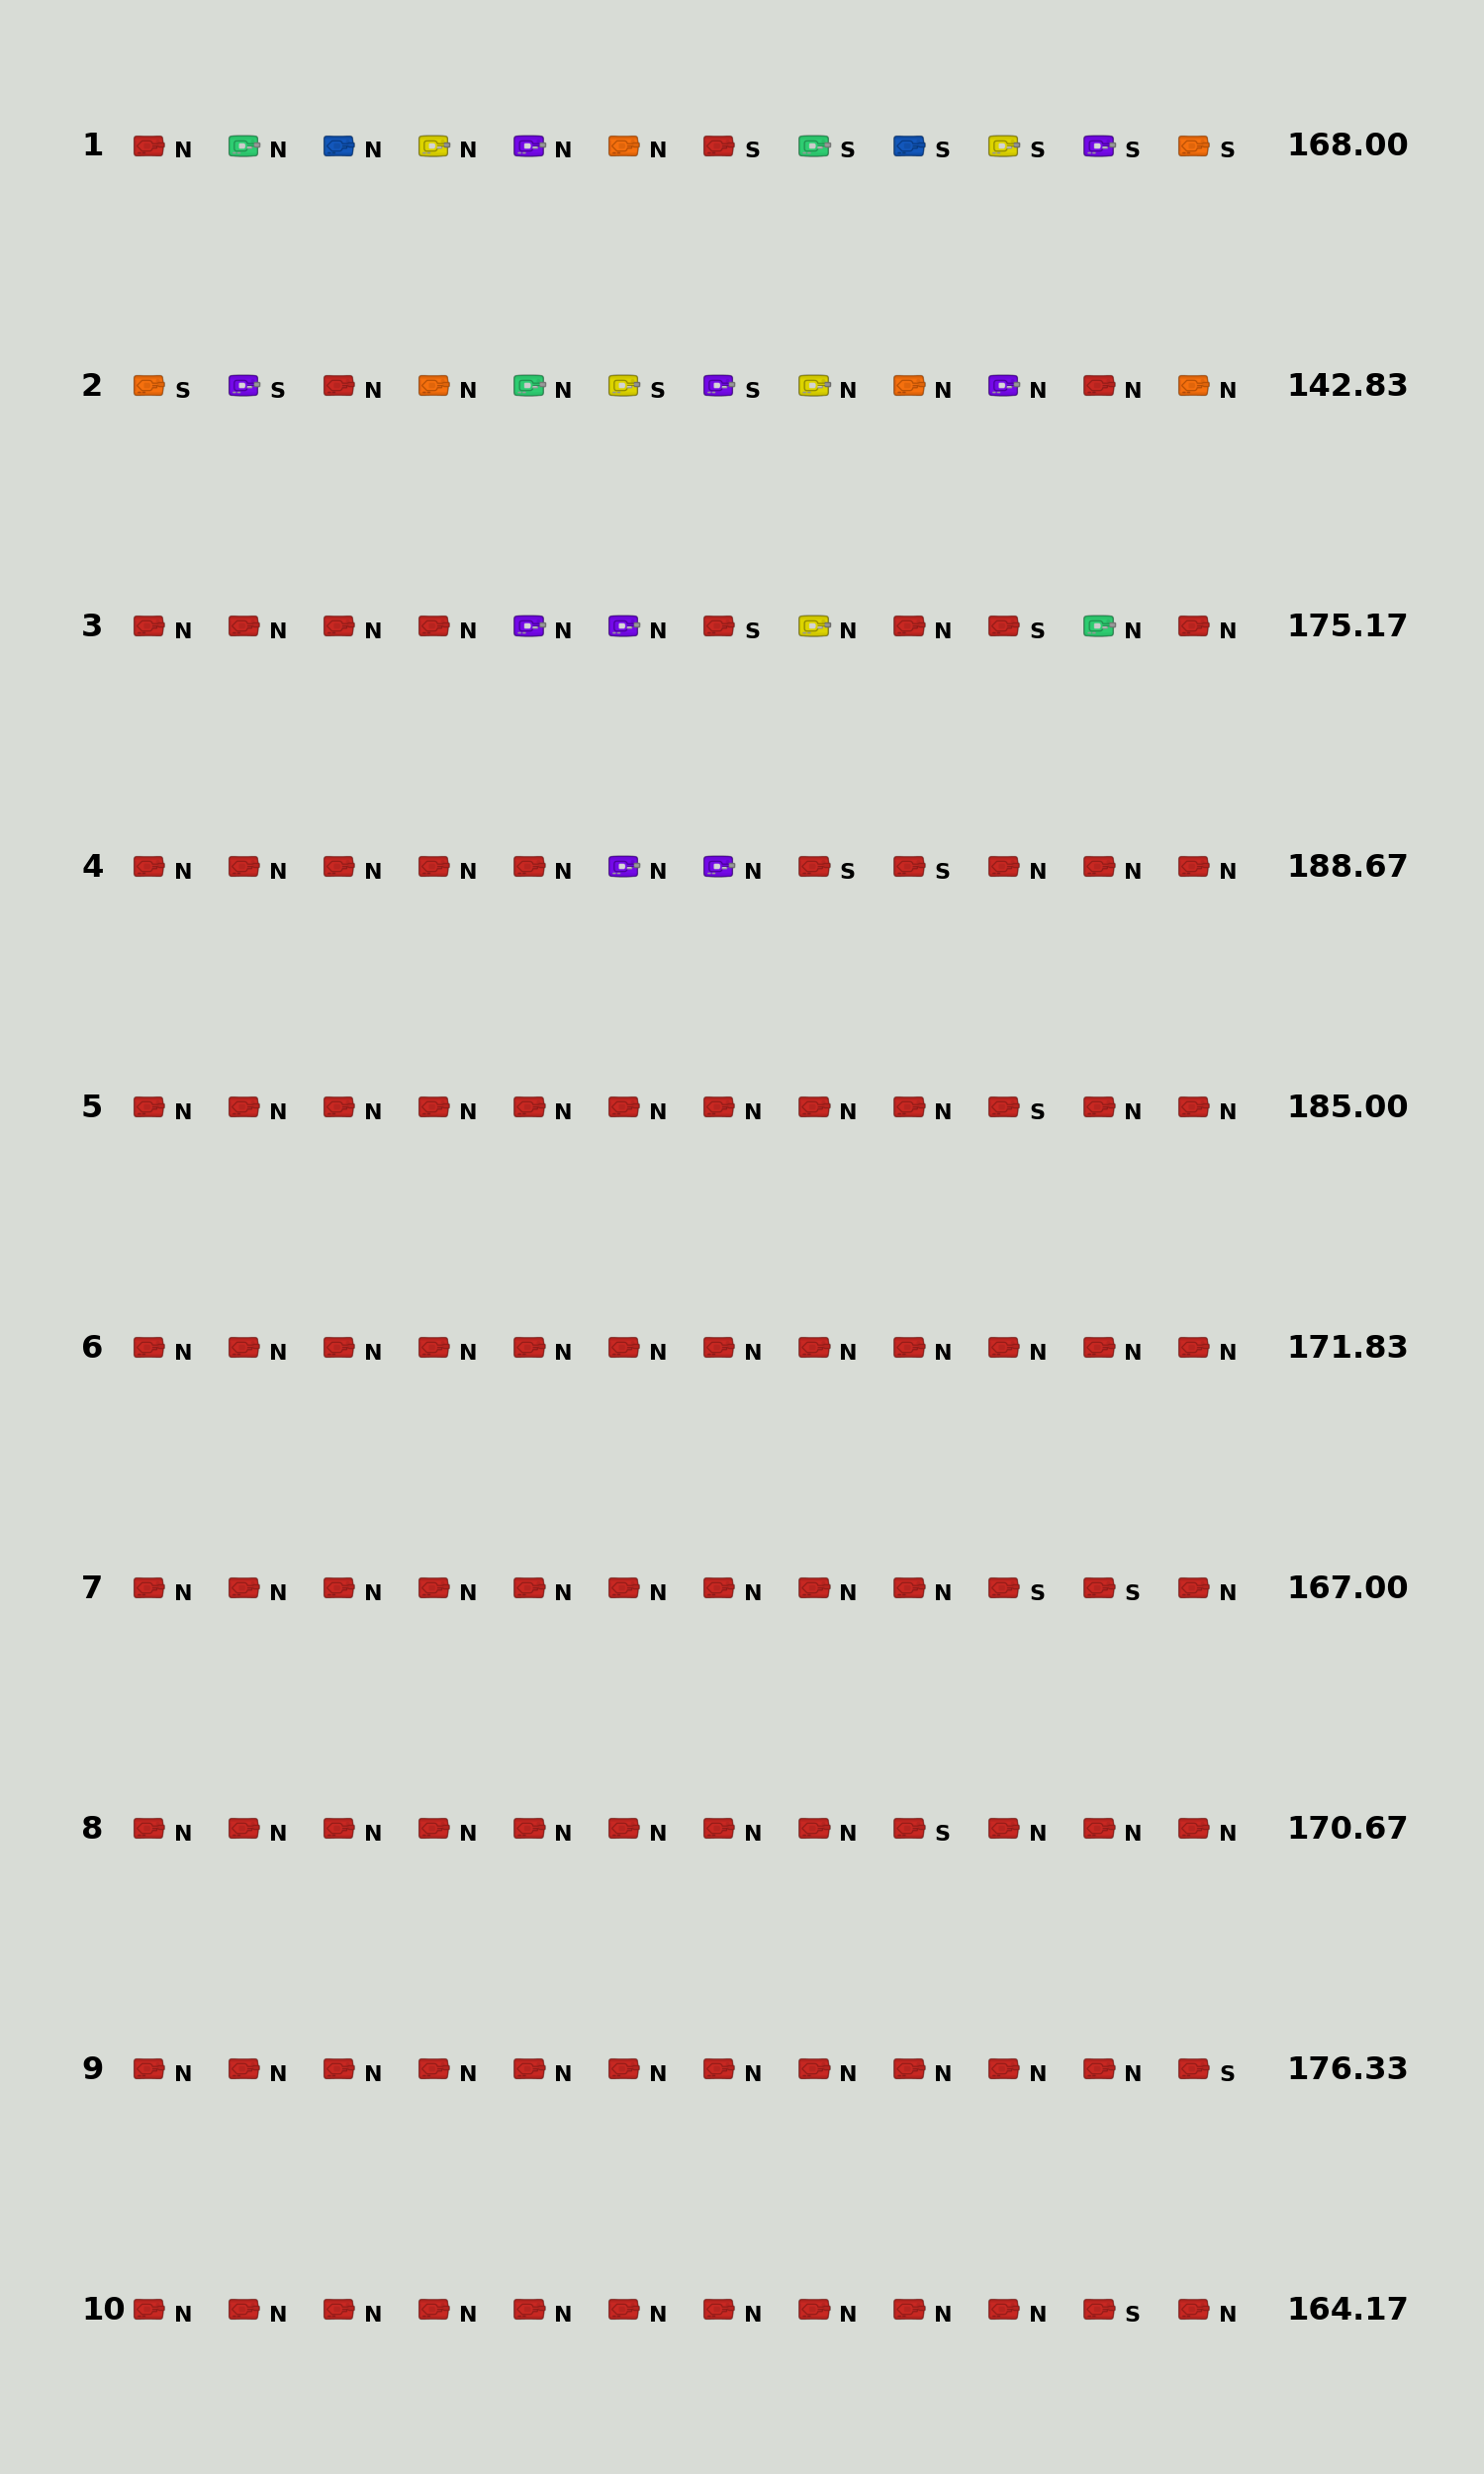
\includegraphics[width=0.9\textwidth]{figuras/td/td_allred_ai_mode_1_1.png}
  \caption{Visualização da moda de cada onda com a versão v1 contra Torres Vermelhas.}
  \label{fig:td-moda-red-1-1}
\end{figure}

\begin{figure}[H]
  \centering
  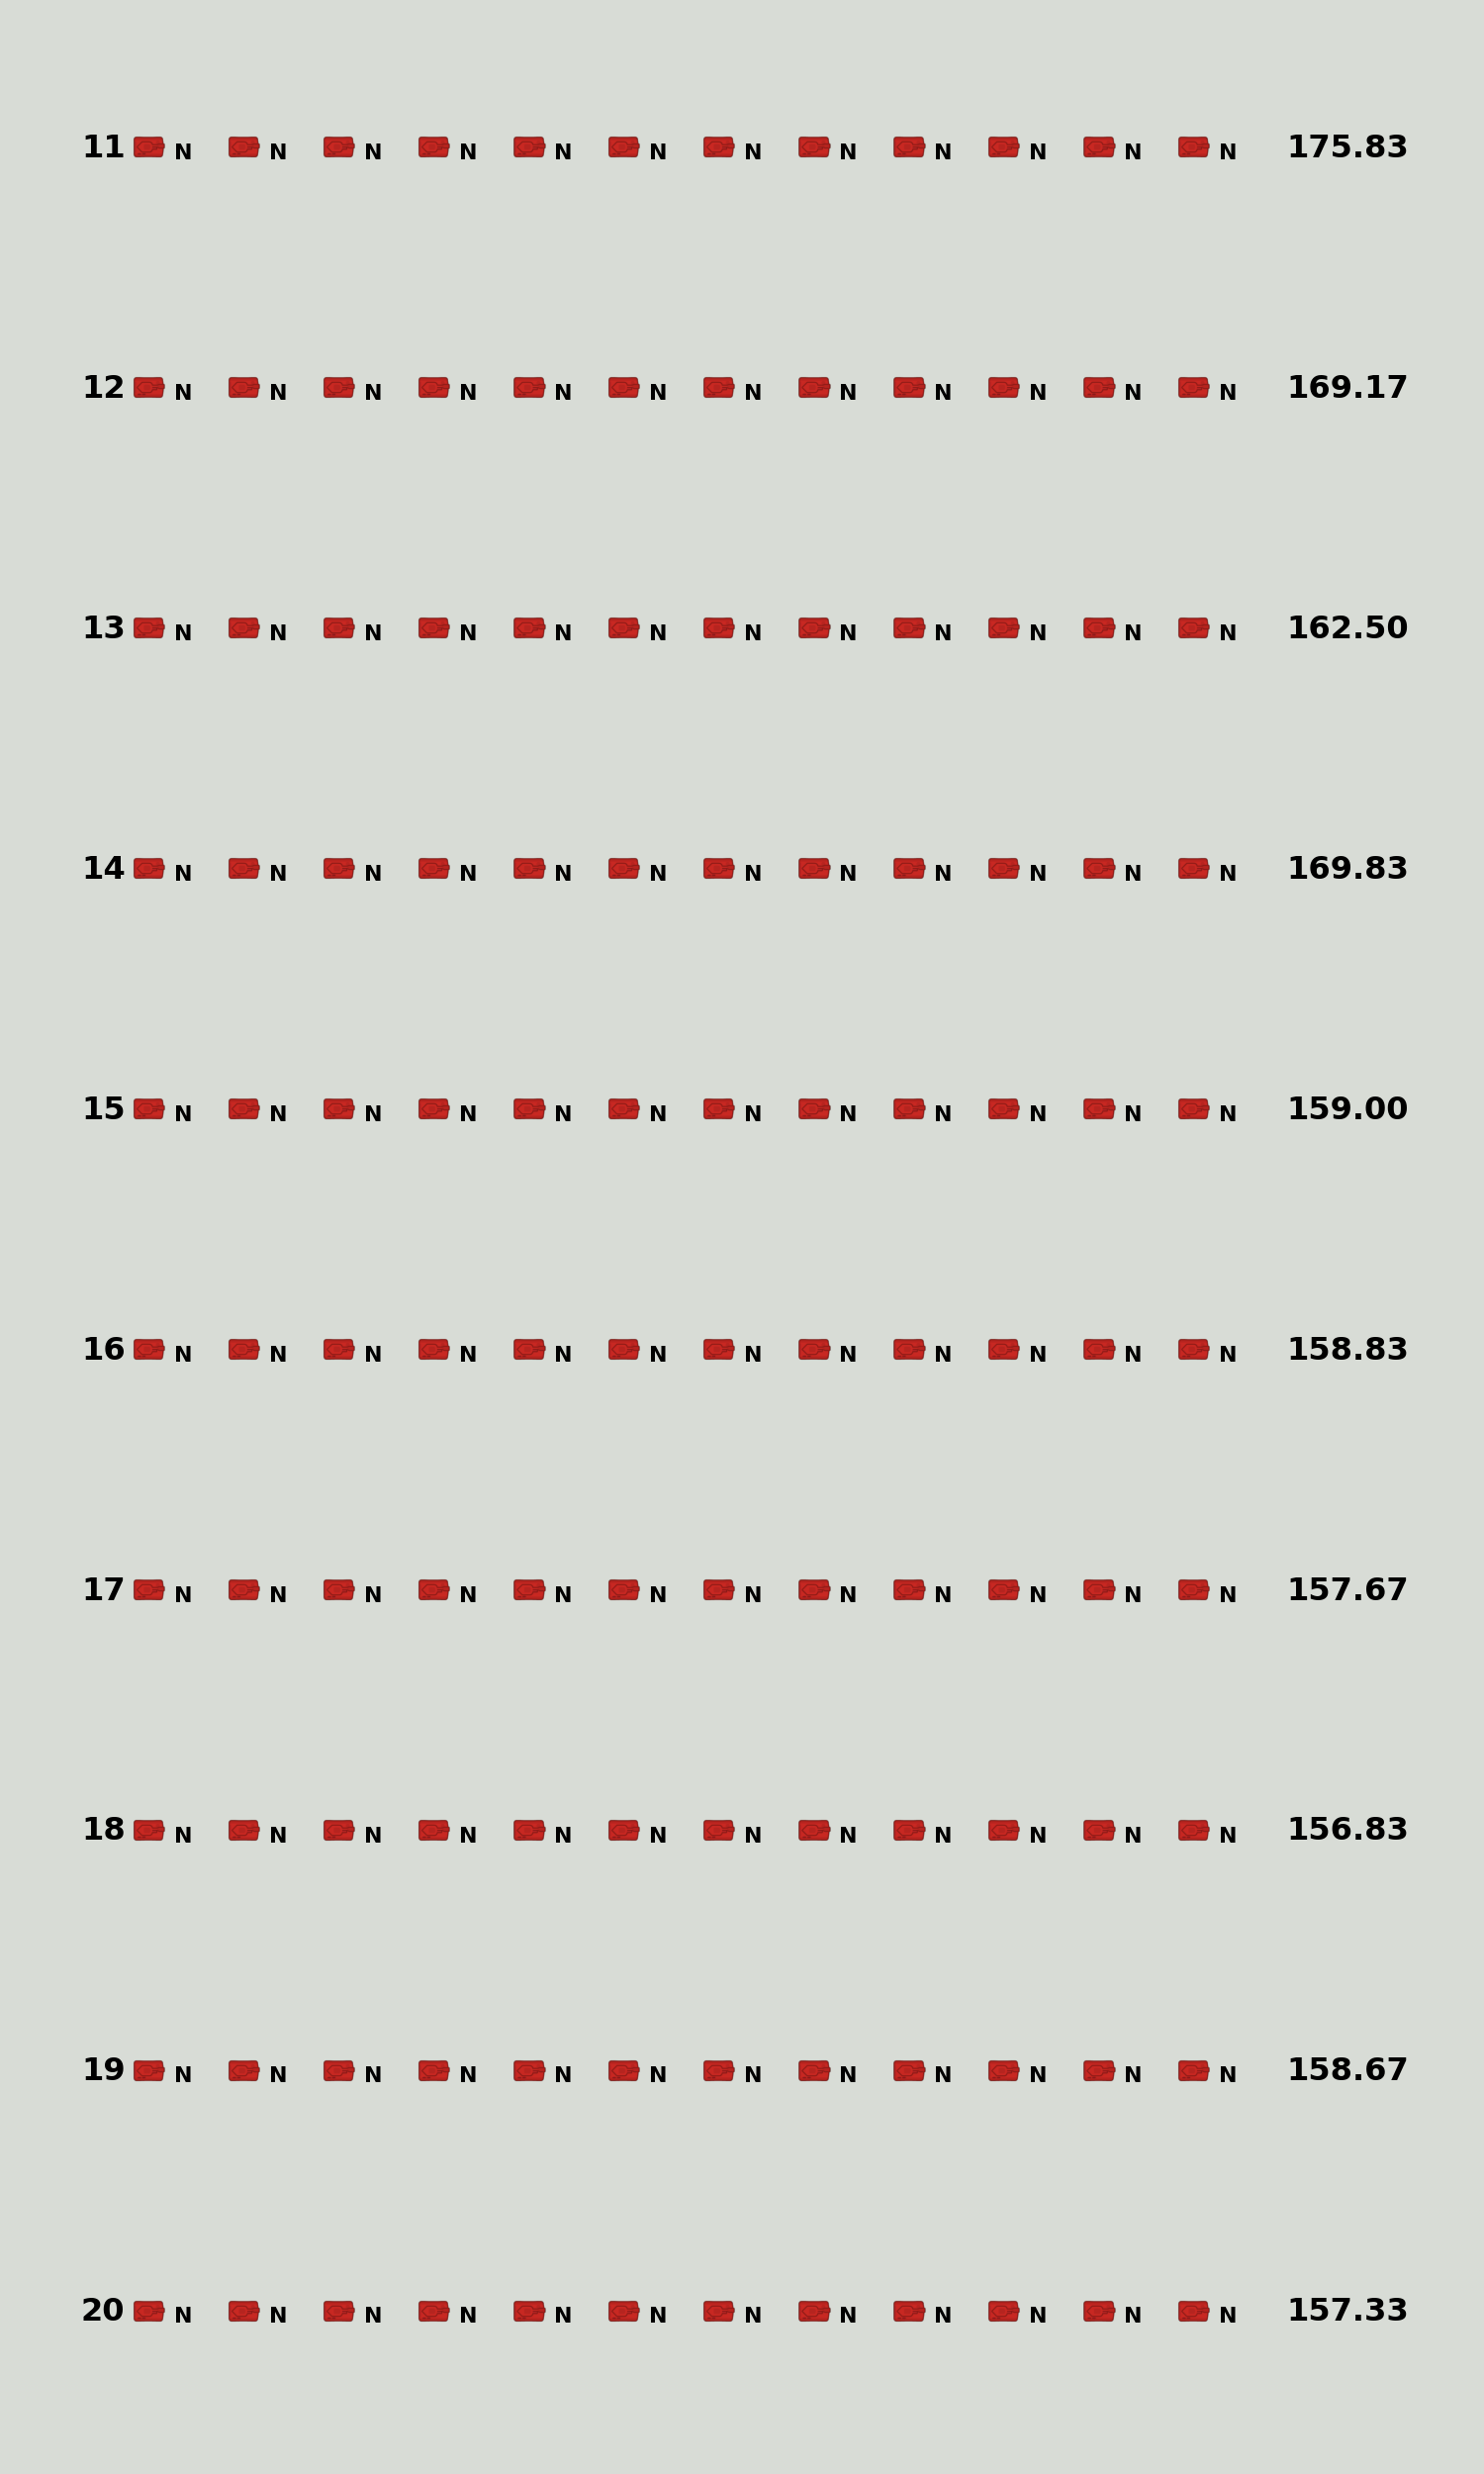
\includegraphics[width=0.9\textwidth]{figuras/td/td_allred_ai_mode_1_2.png}
  \caption{Visualização da moda de cada onda com a versão v1 contra Torres Vermelhas.}
  \label{fig:td-moda-red-1-2}
\end{figure}

\begin{figure}[H]
  \centering
  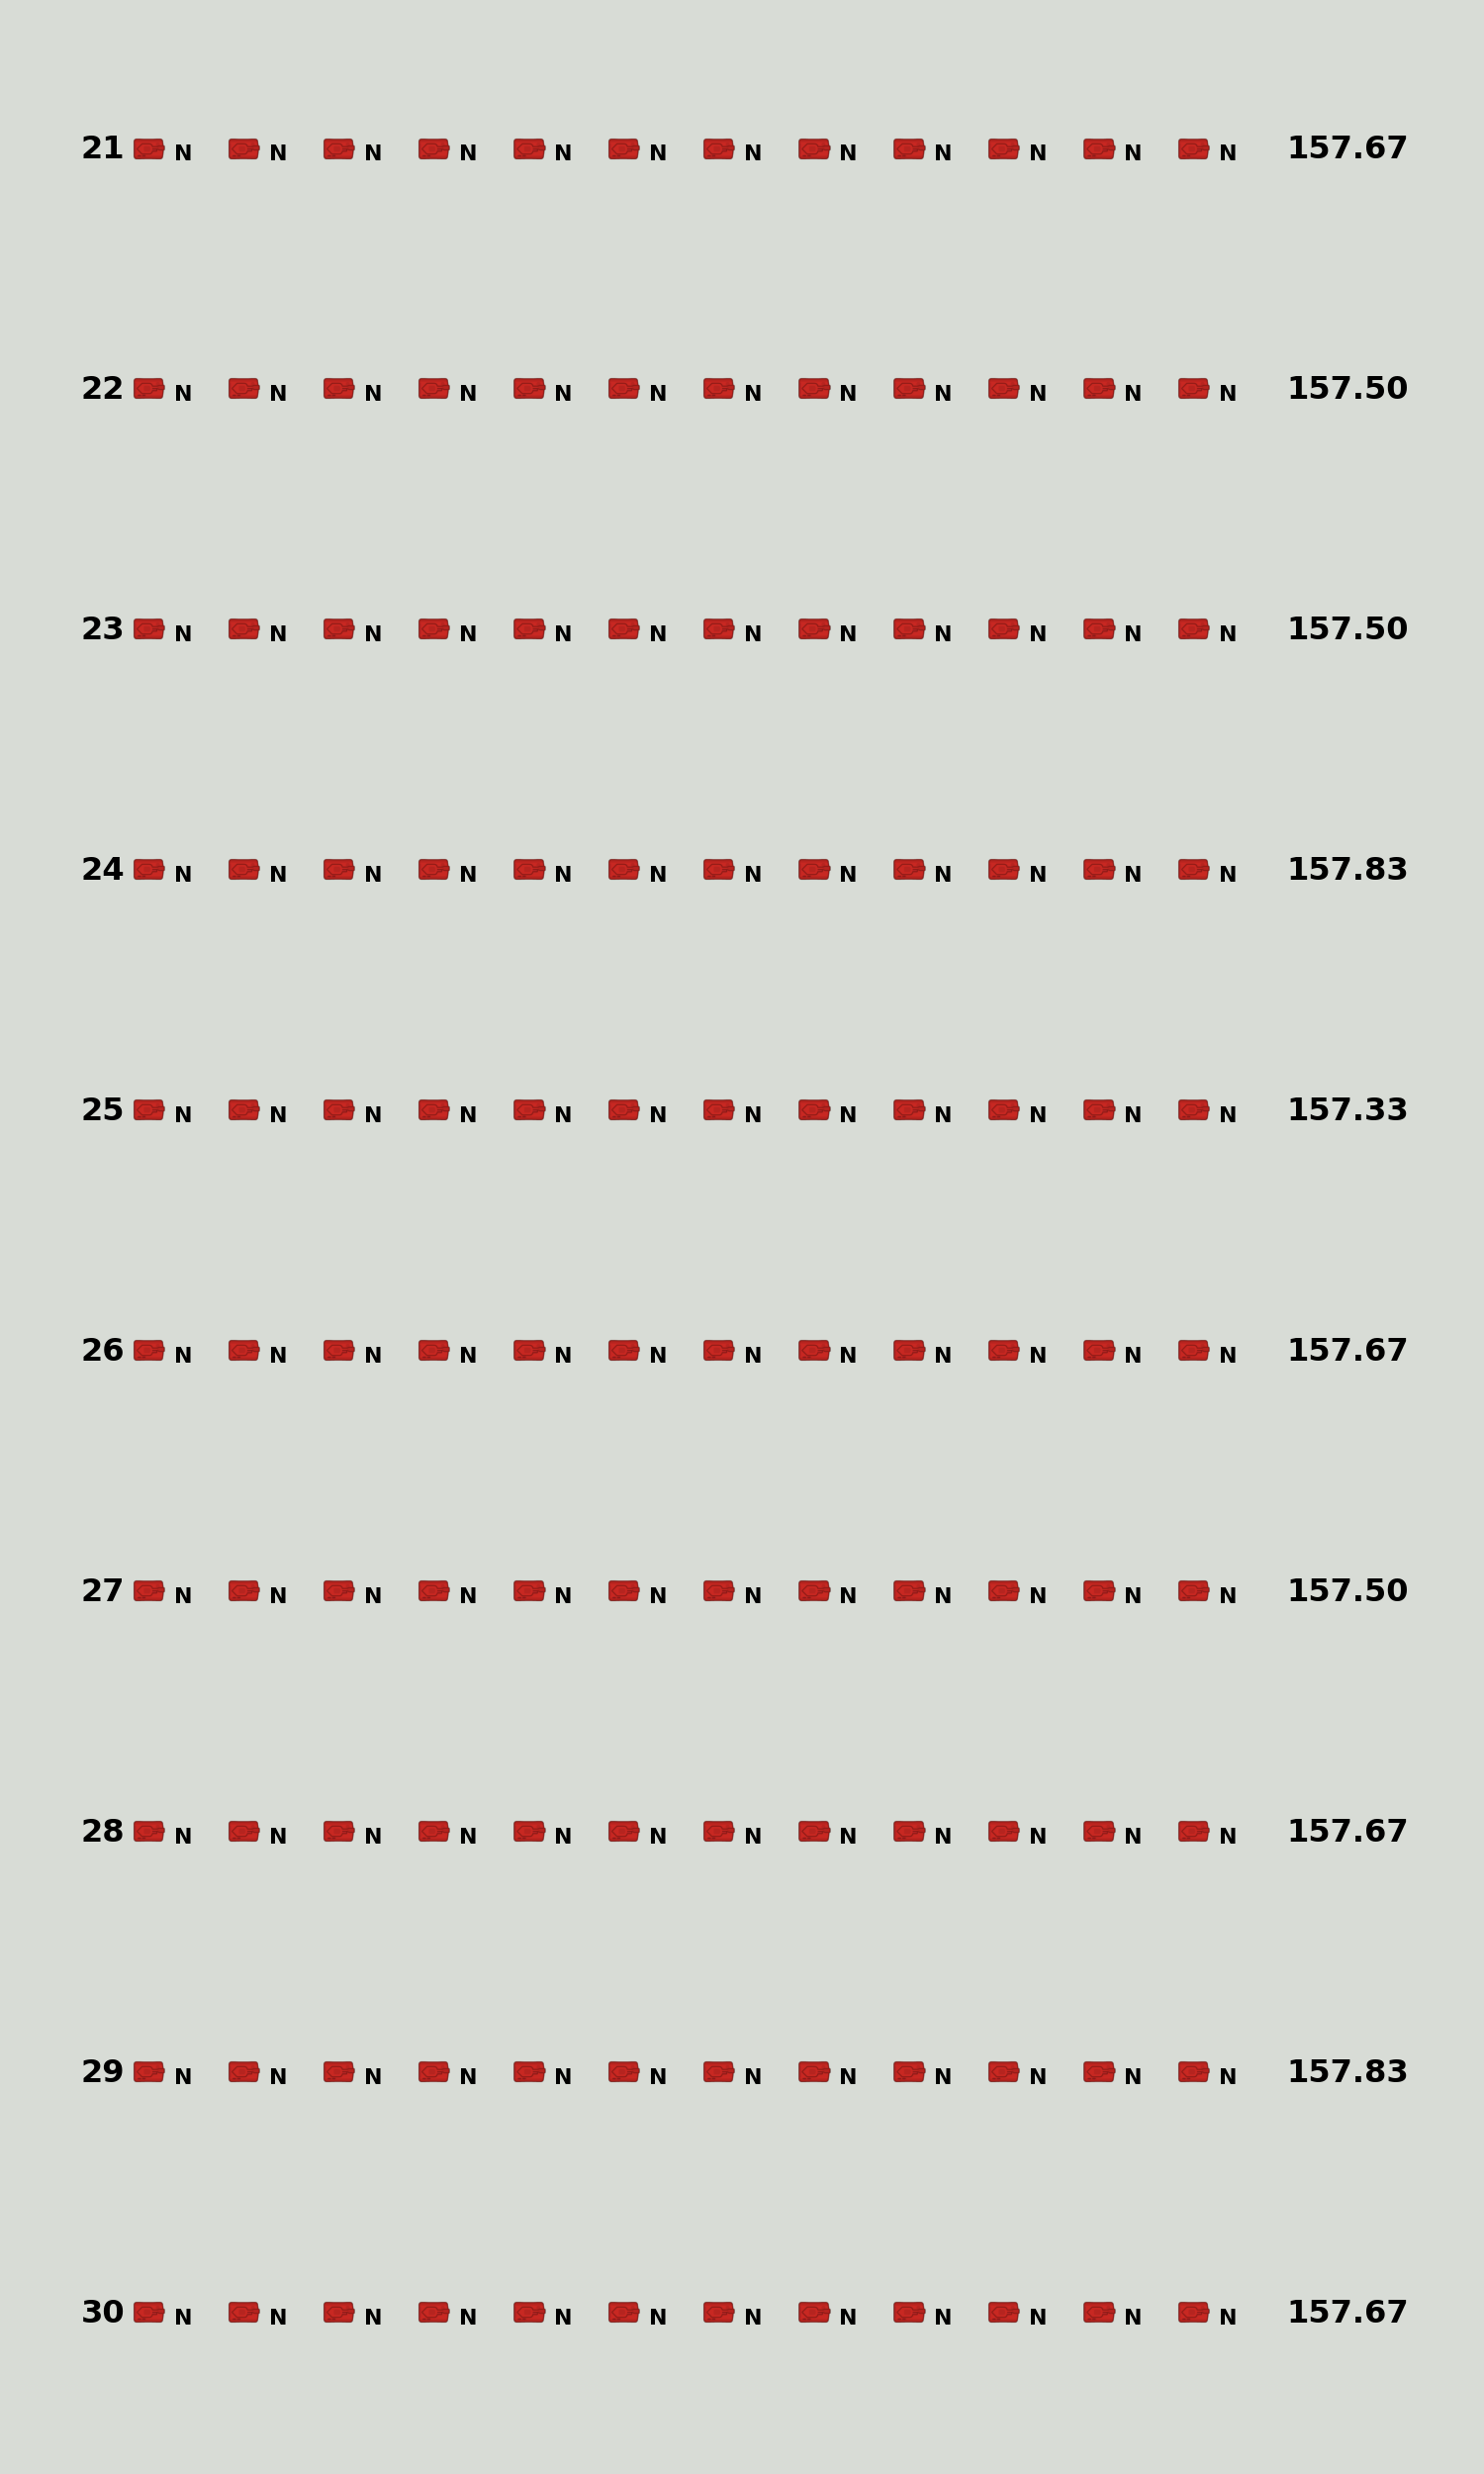
\includegraphics[width=0.9\textwidth]{figuras/td/td_allred_ai_mode_1_3.png}
  \caption{Visualização da moda de cada onda com a versão v1 contra Torres Vermelhas.}
  \label{fig:td-moda-red-1-3}
\end{figure}

%% ------------------------------------------------------------------------- %%
\section{Torres Verde + Vermelha}
\label{sec:apend-moda-td-gr-v1}

\begin{figure}[H]
  \centering
  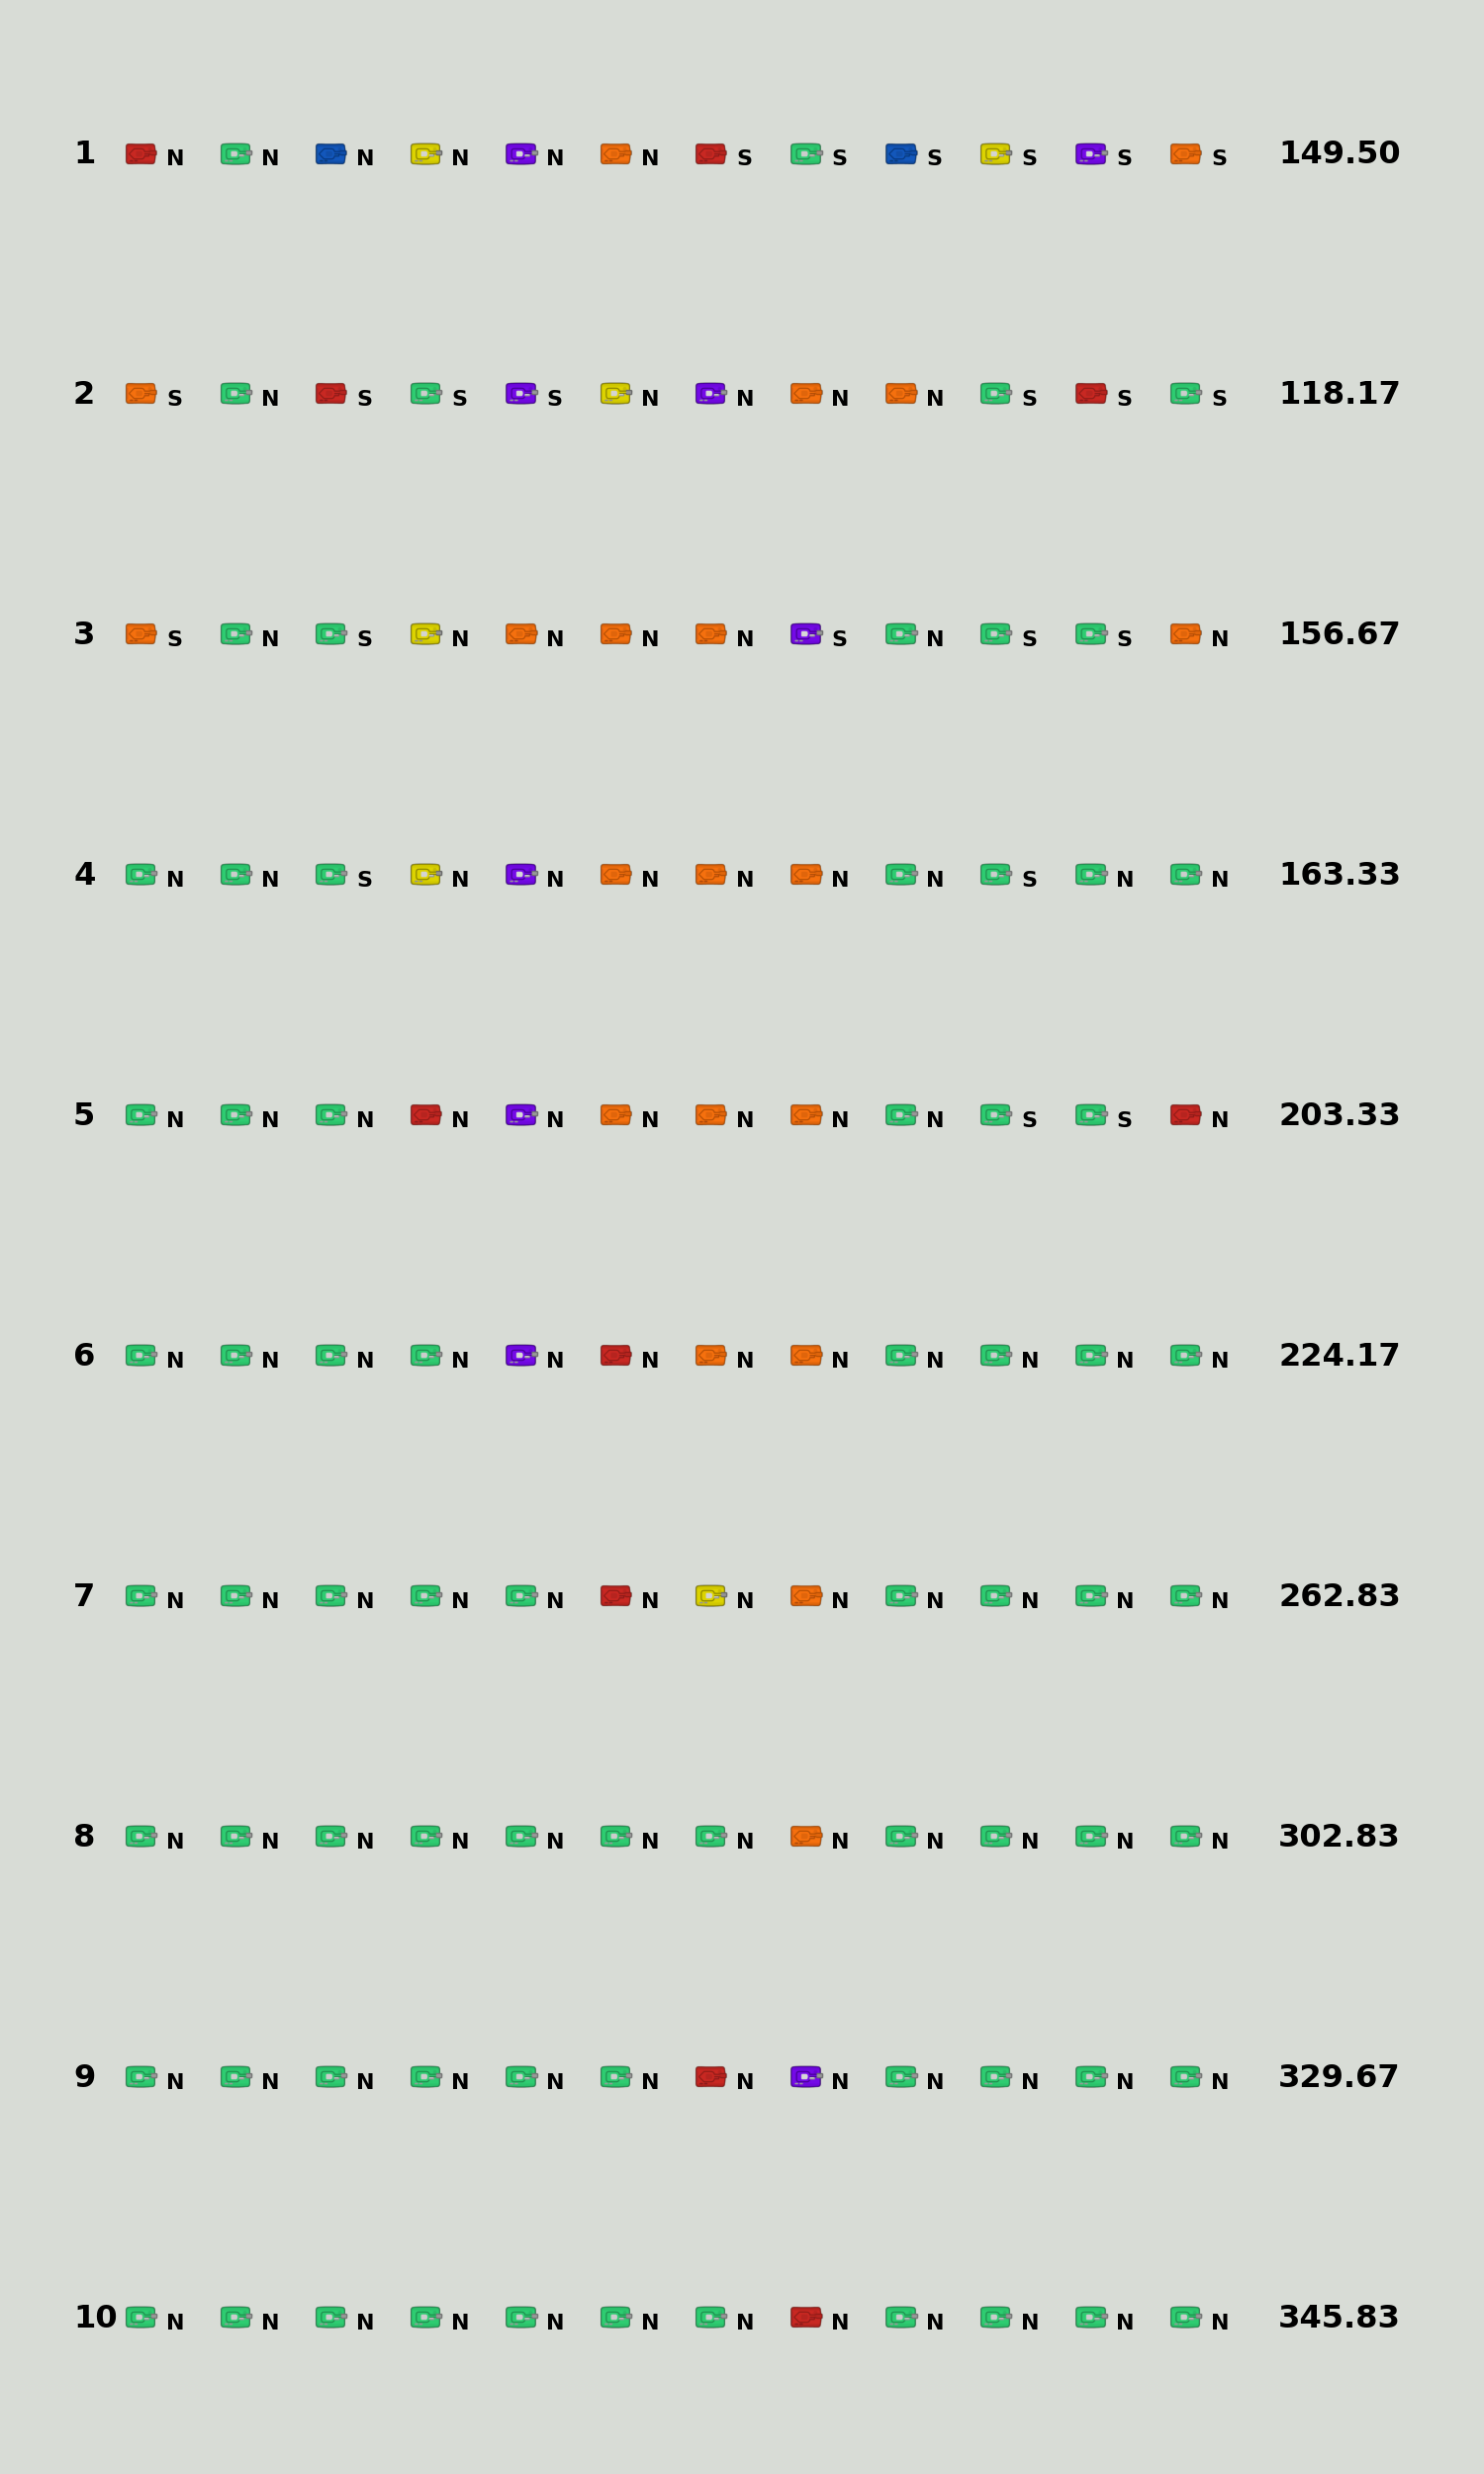
\includegraphics[width=0.9\textwidth]{figuras/td/td_greenred_ai_mode_1_1.png}
  \caption{Visualização da moda de cada onda com a versão v1 contra Torres Verdes + Vermelhas.}
  \label{fig:td-moda-greenred-1-1}
\end{figure}

\begin{figure}[H]
  \centering
  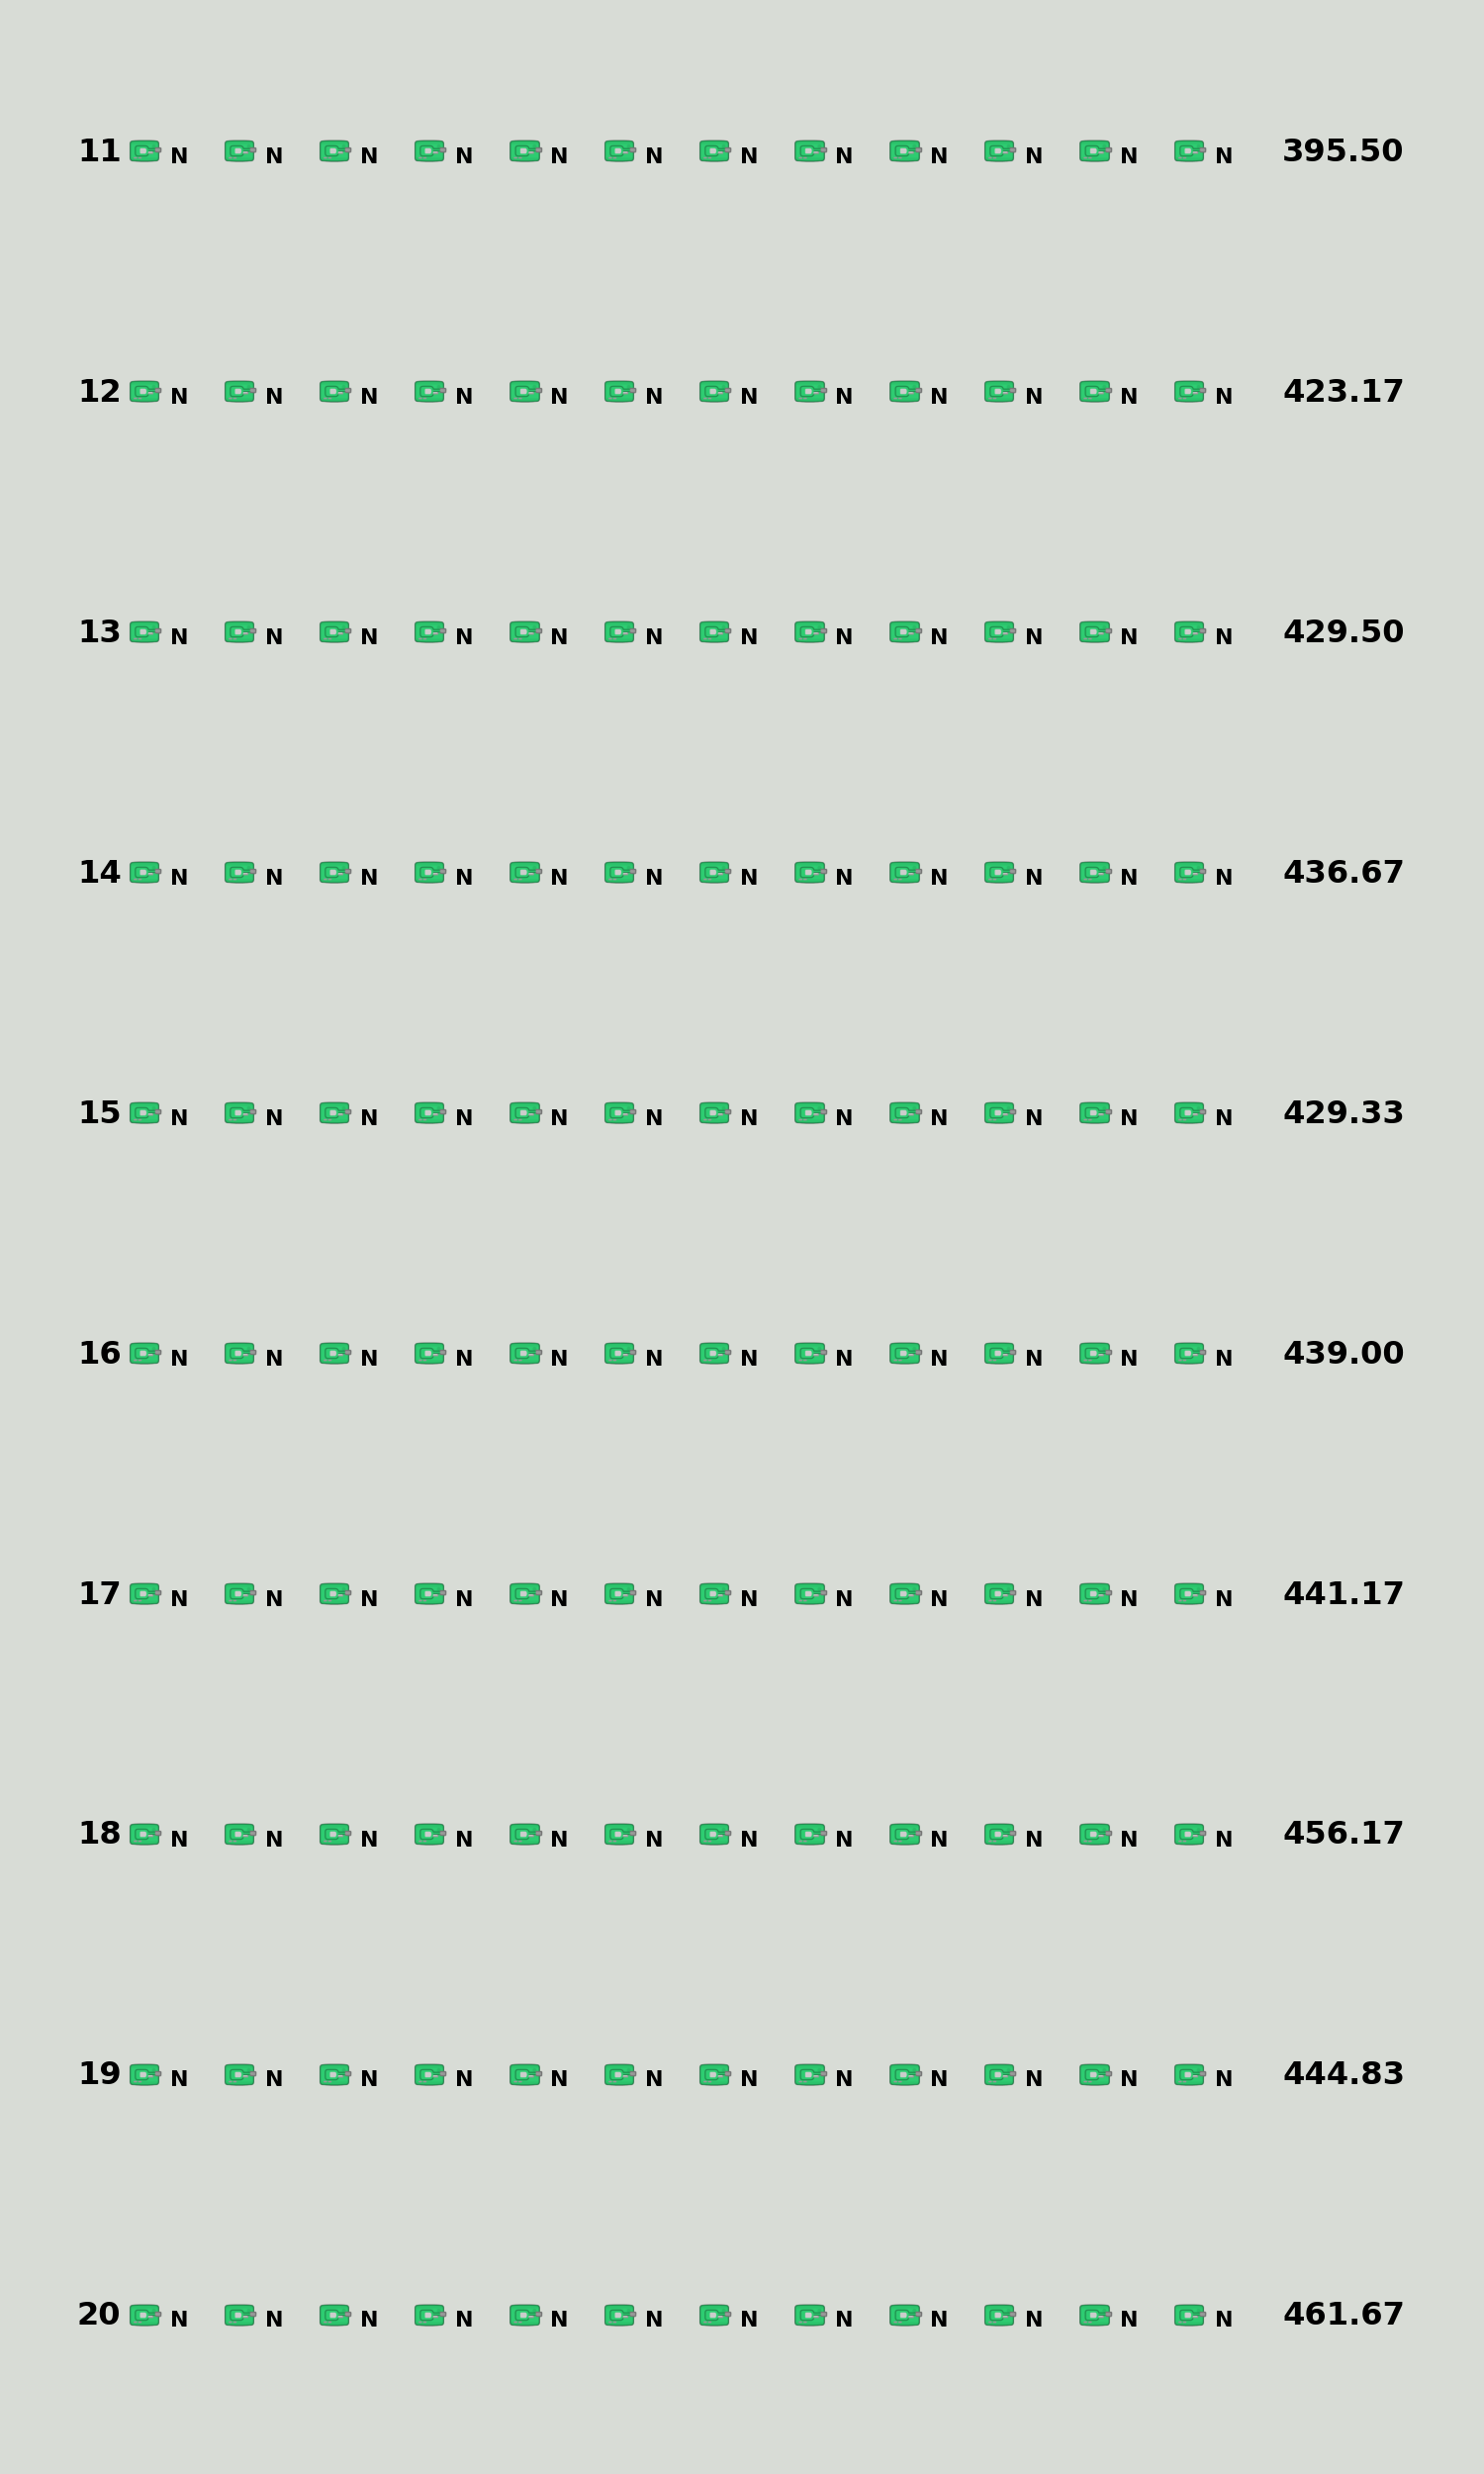
\includegraphics[width=0.9\textwidth]{figuras/td/td_greenred_ai_mode_1_2.png}
  \caption{Visualização da moda de cada onda com a versão v1 contra Torres Verdes + Vermelhas.}
  \label{fig:td-moda-greenred-1-2}
\end{figure}

\begin{figure}[H]
  \centering
  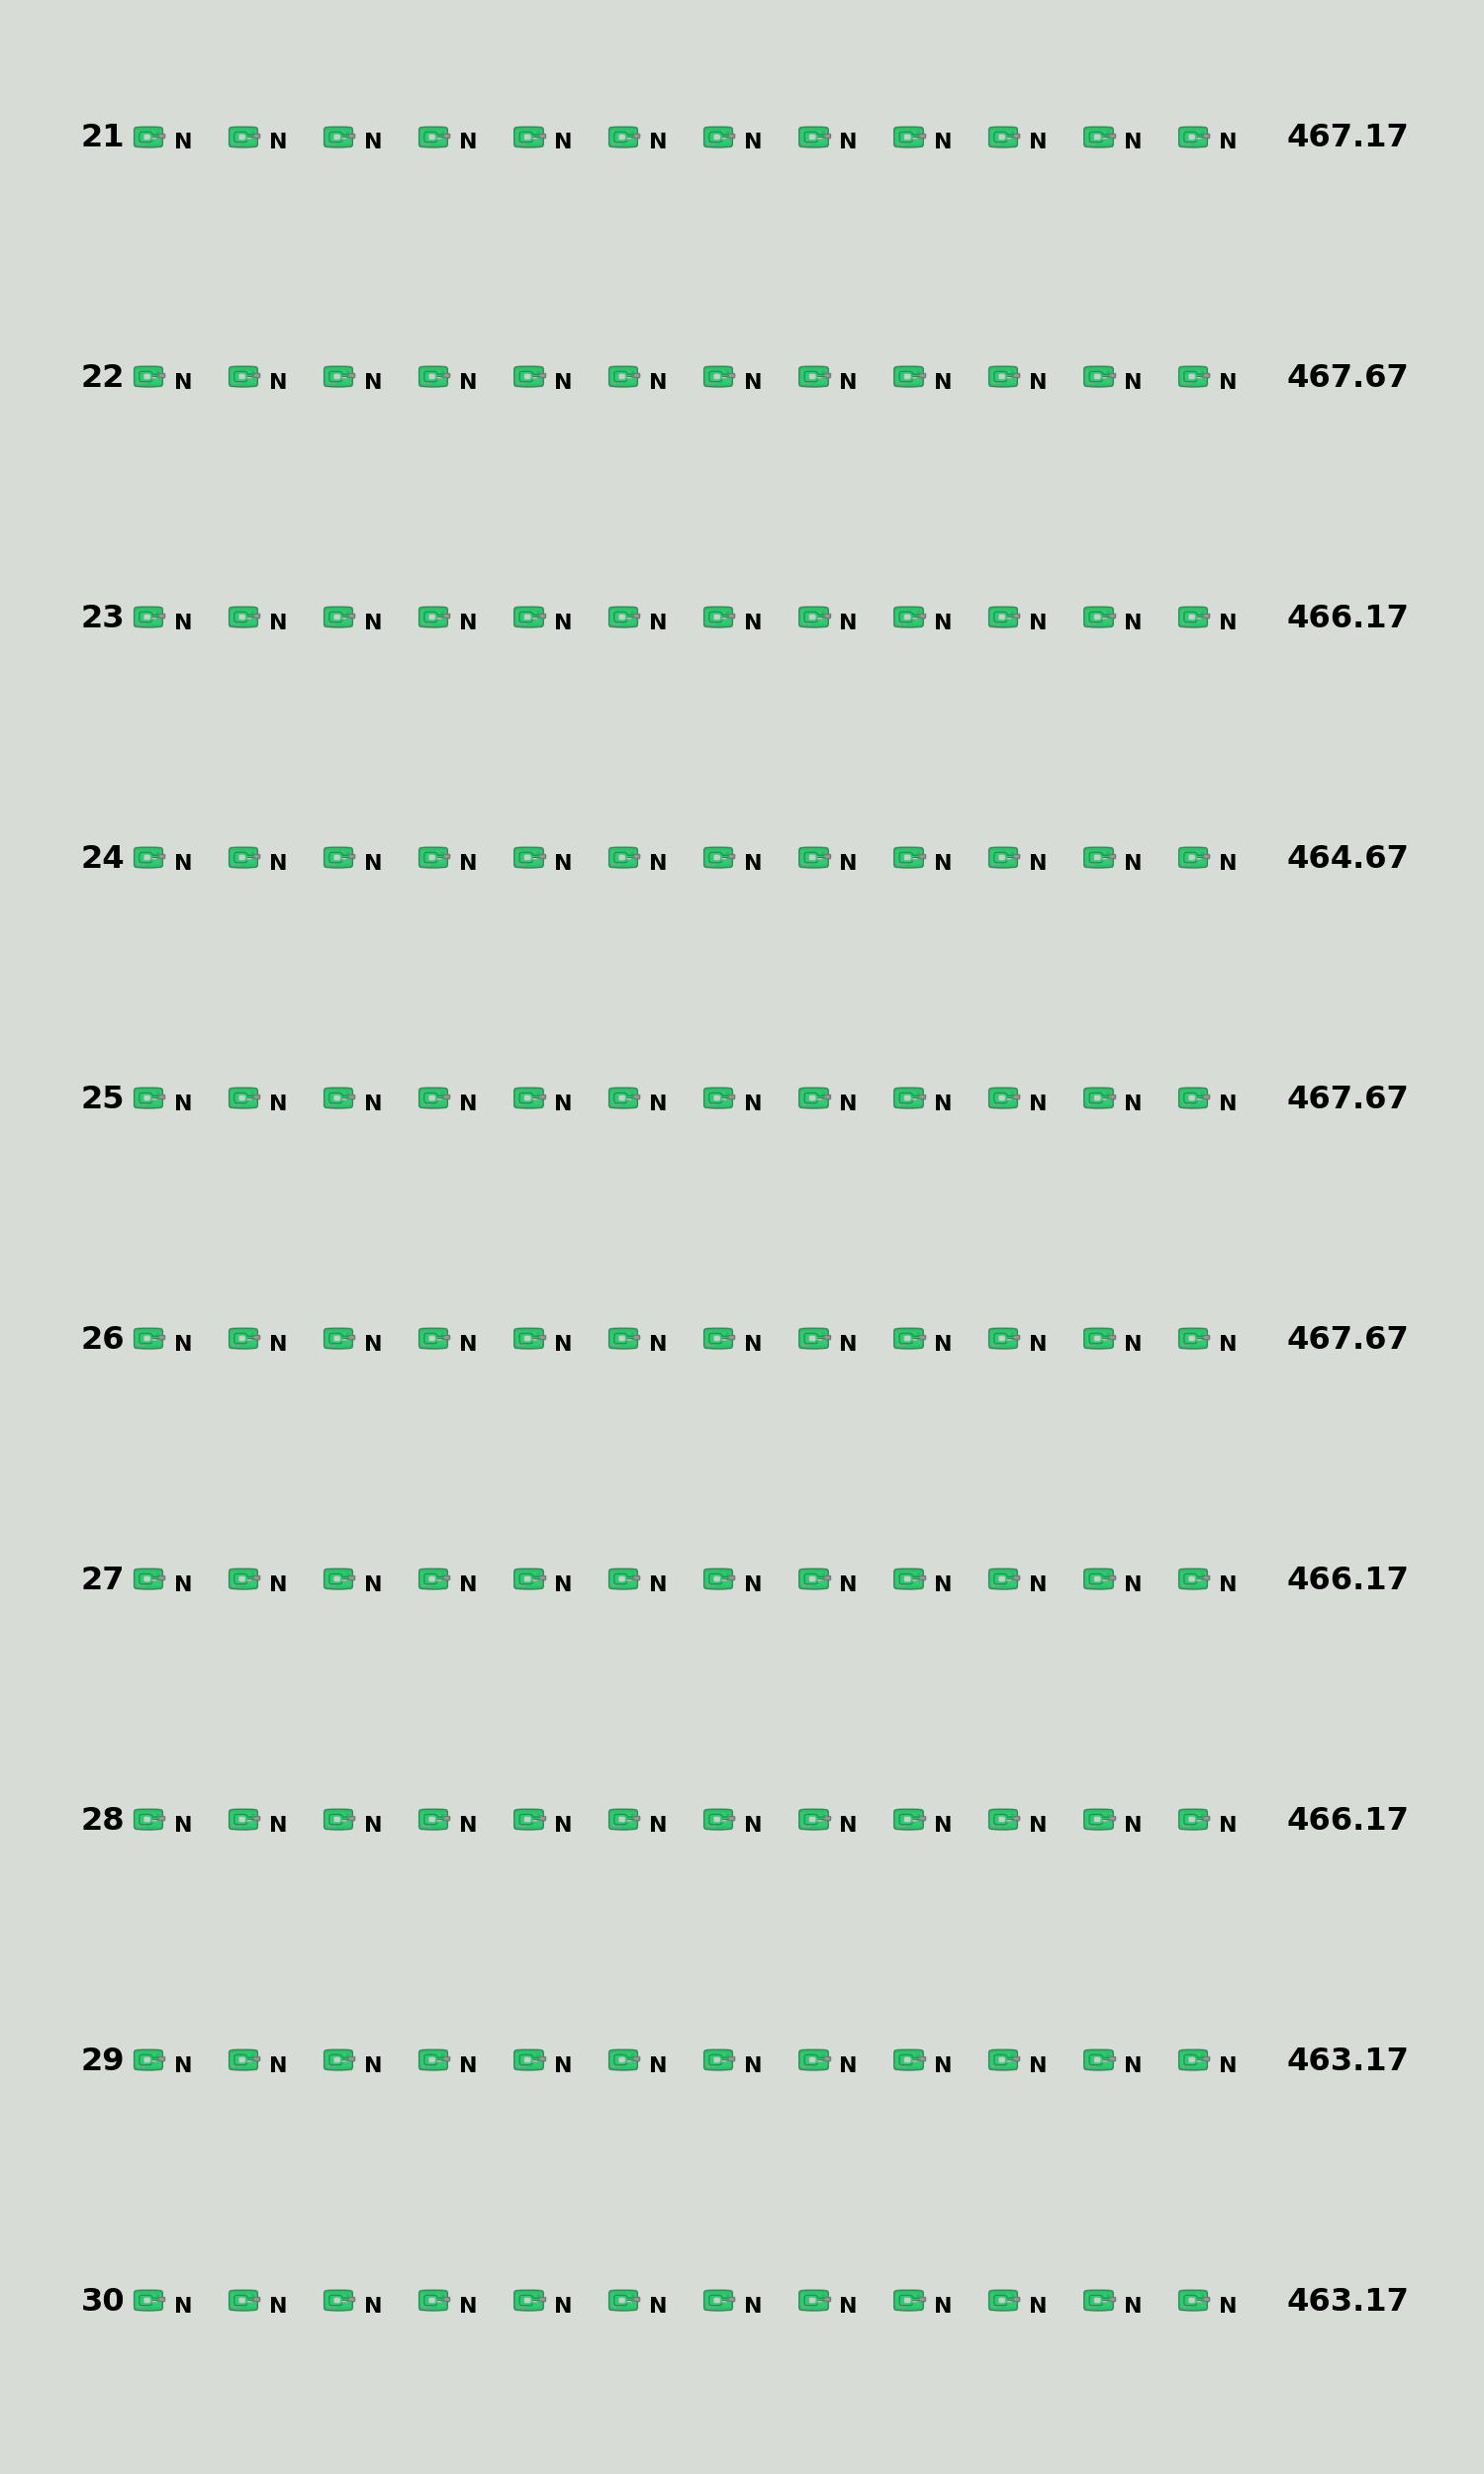
\includegraphics[width=0.9\textwidth]{figuras/td/td_greenred_ai_mode_1_3.png}
  \caption{Visualização da moda de cada onda com a versão v1 contra Torres Verdes + Vermelhas.}
  \label{fig:td-moda-greenred-1-3}
\end{figure}

%% ------------------------------------------------------------------------- %%
\section{Torres Vermelha + Verde}
\label{sec:apend-moda-td-rg-v1}

\begin{figure}[H]
  \centering
  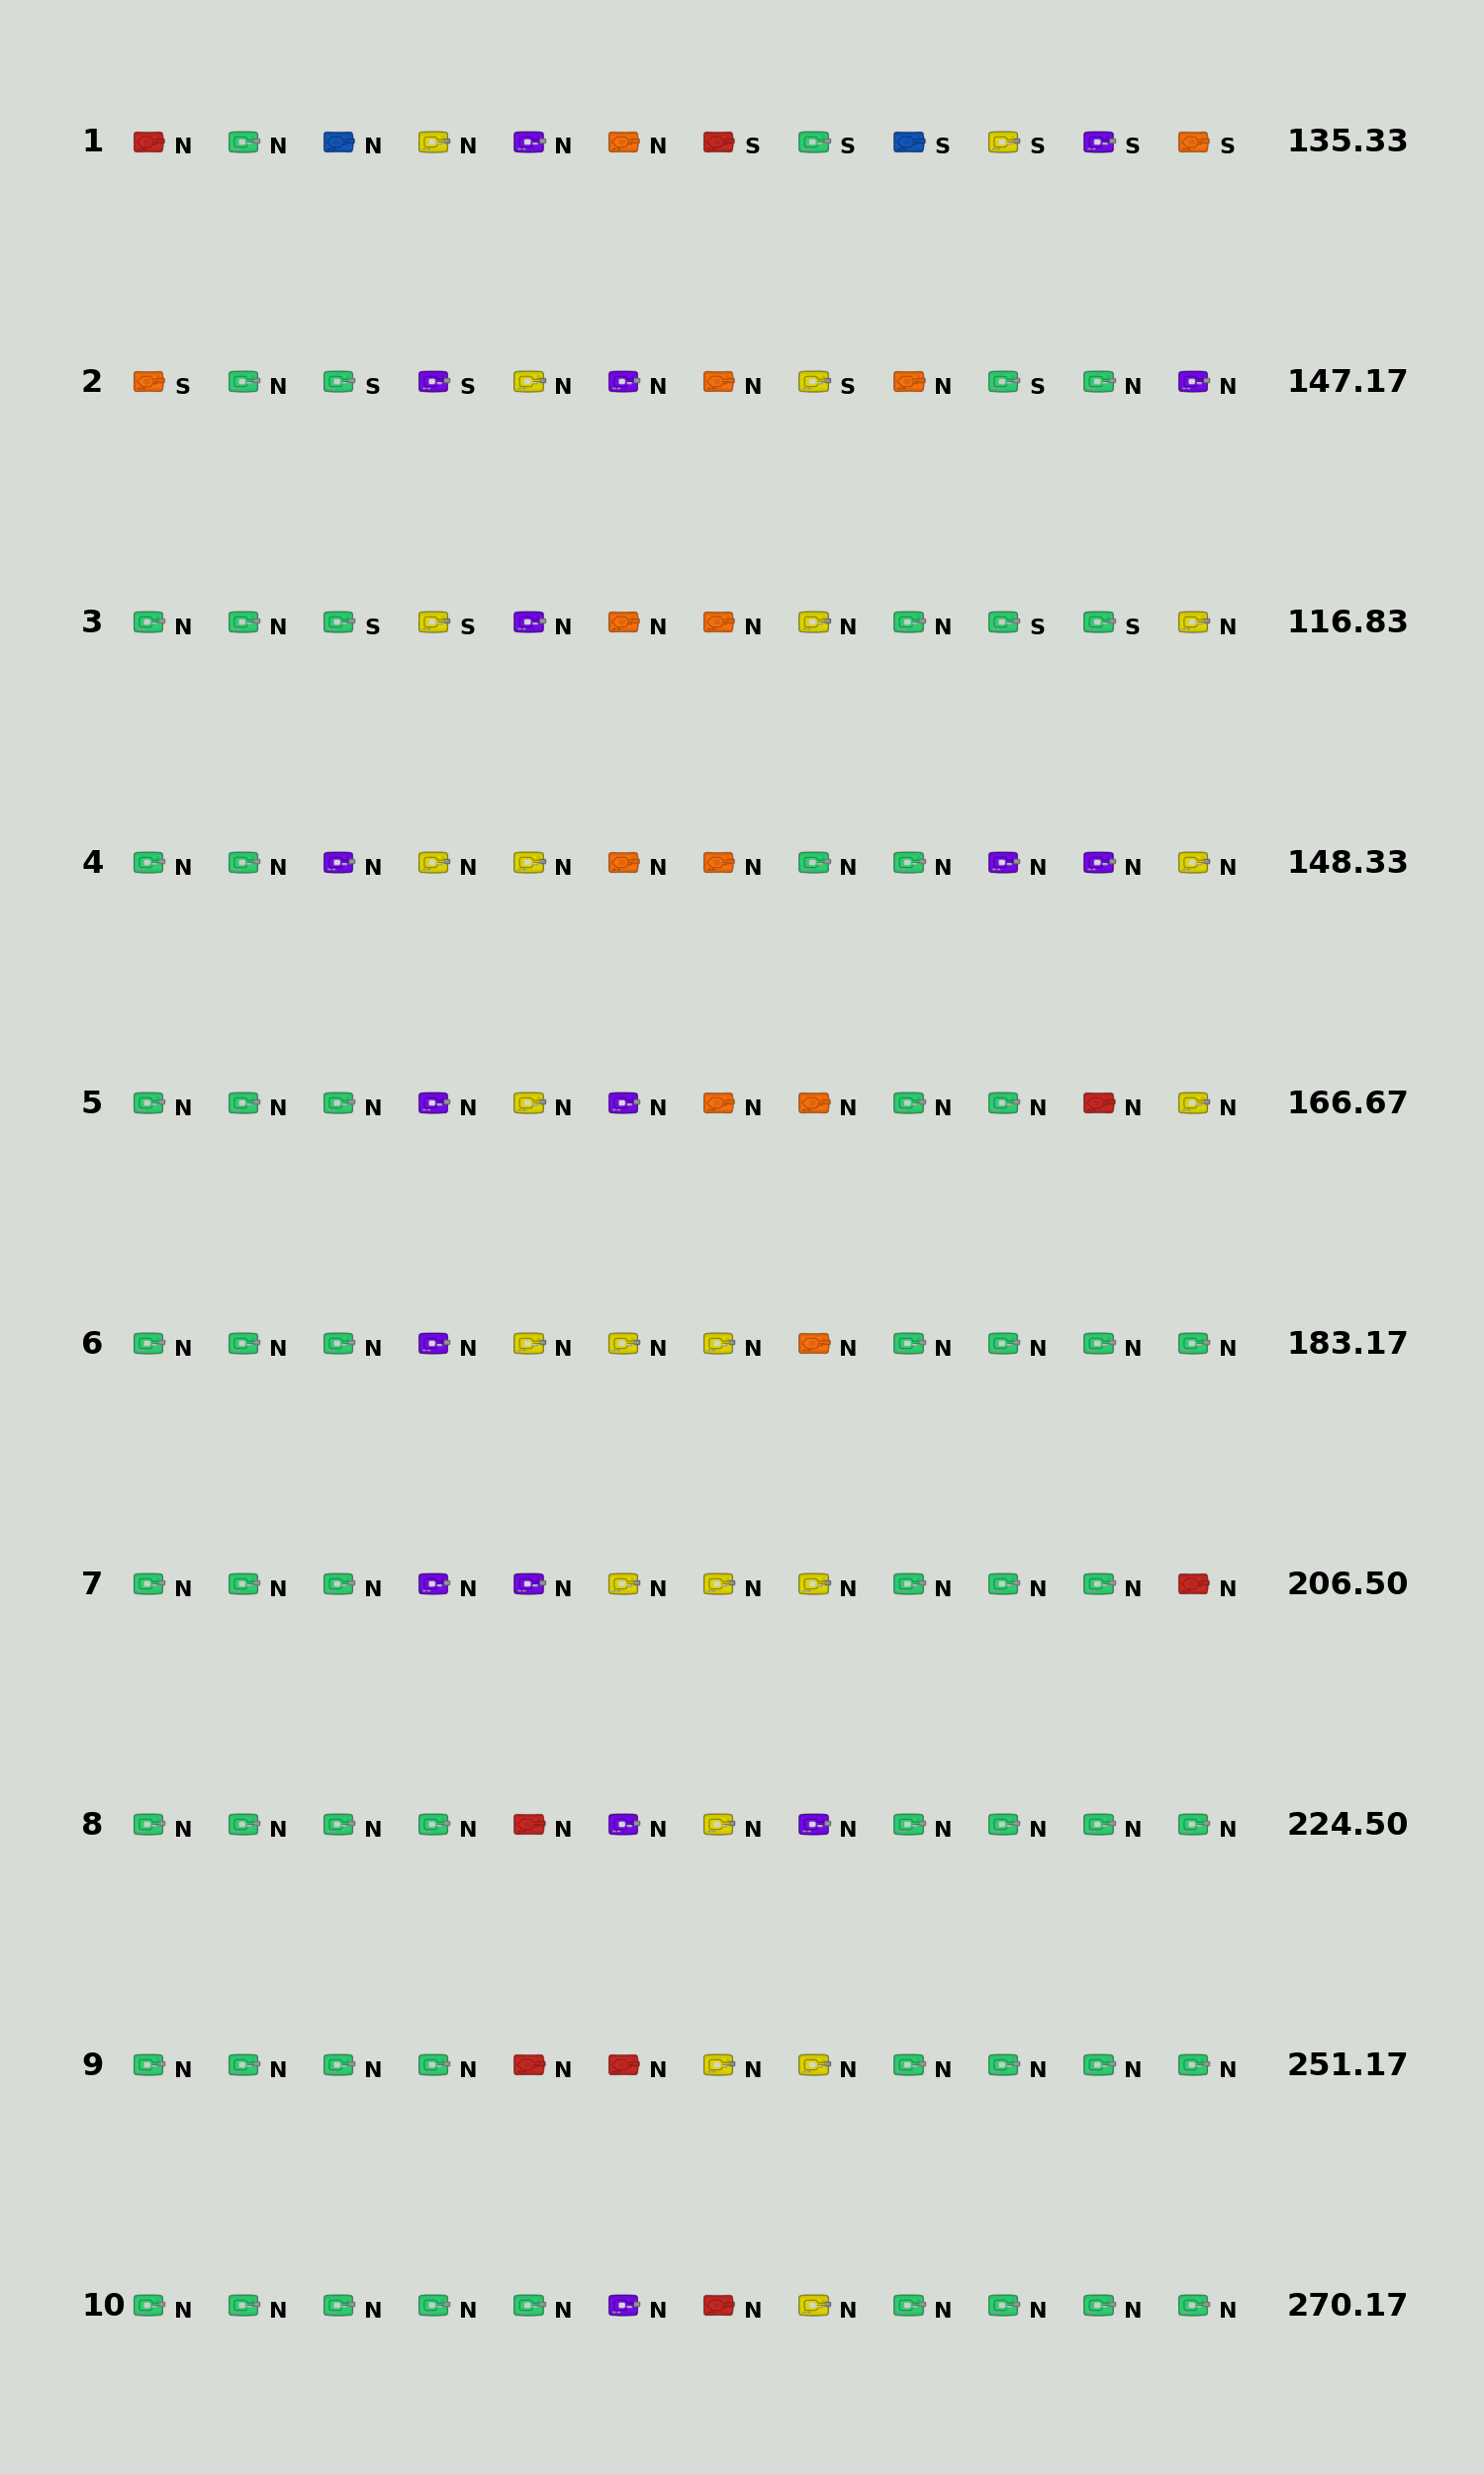
\includegraphics[width=0.9\textwidth]{figuras/td/td_redgreen_ai_mode_1_1.png}
  \caption{Visualização da moda de cada onda com a versão v1 contra Torres Vermelhas + Verdes.}
  \label{fig:td-moda-redgreen-1-1}
\end{figure}

\begin{figure}[H]
  \centering
  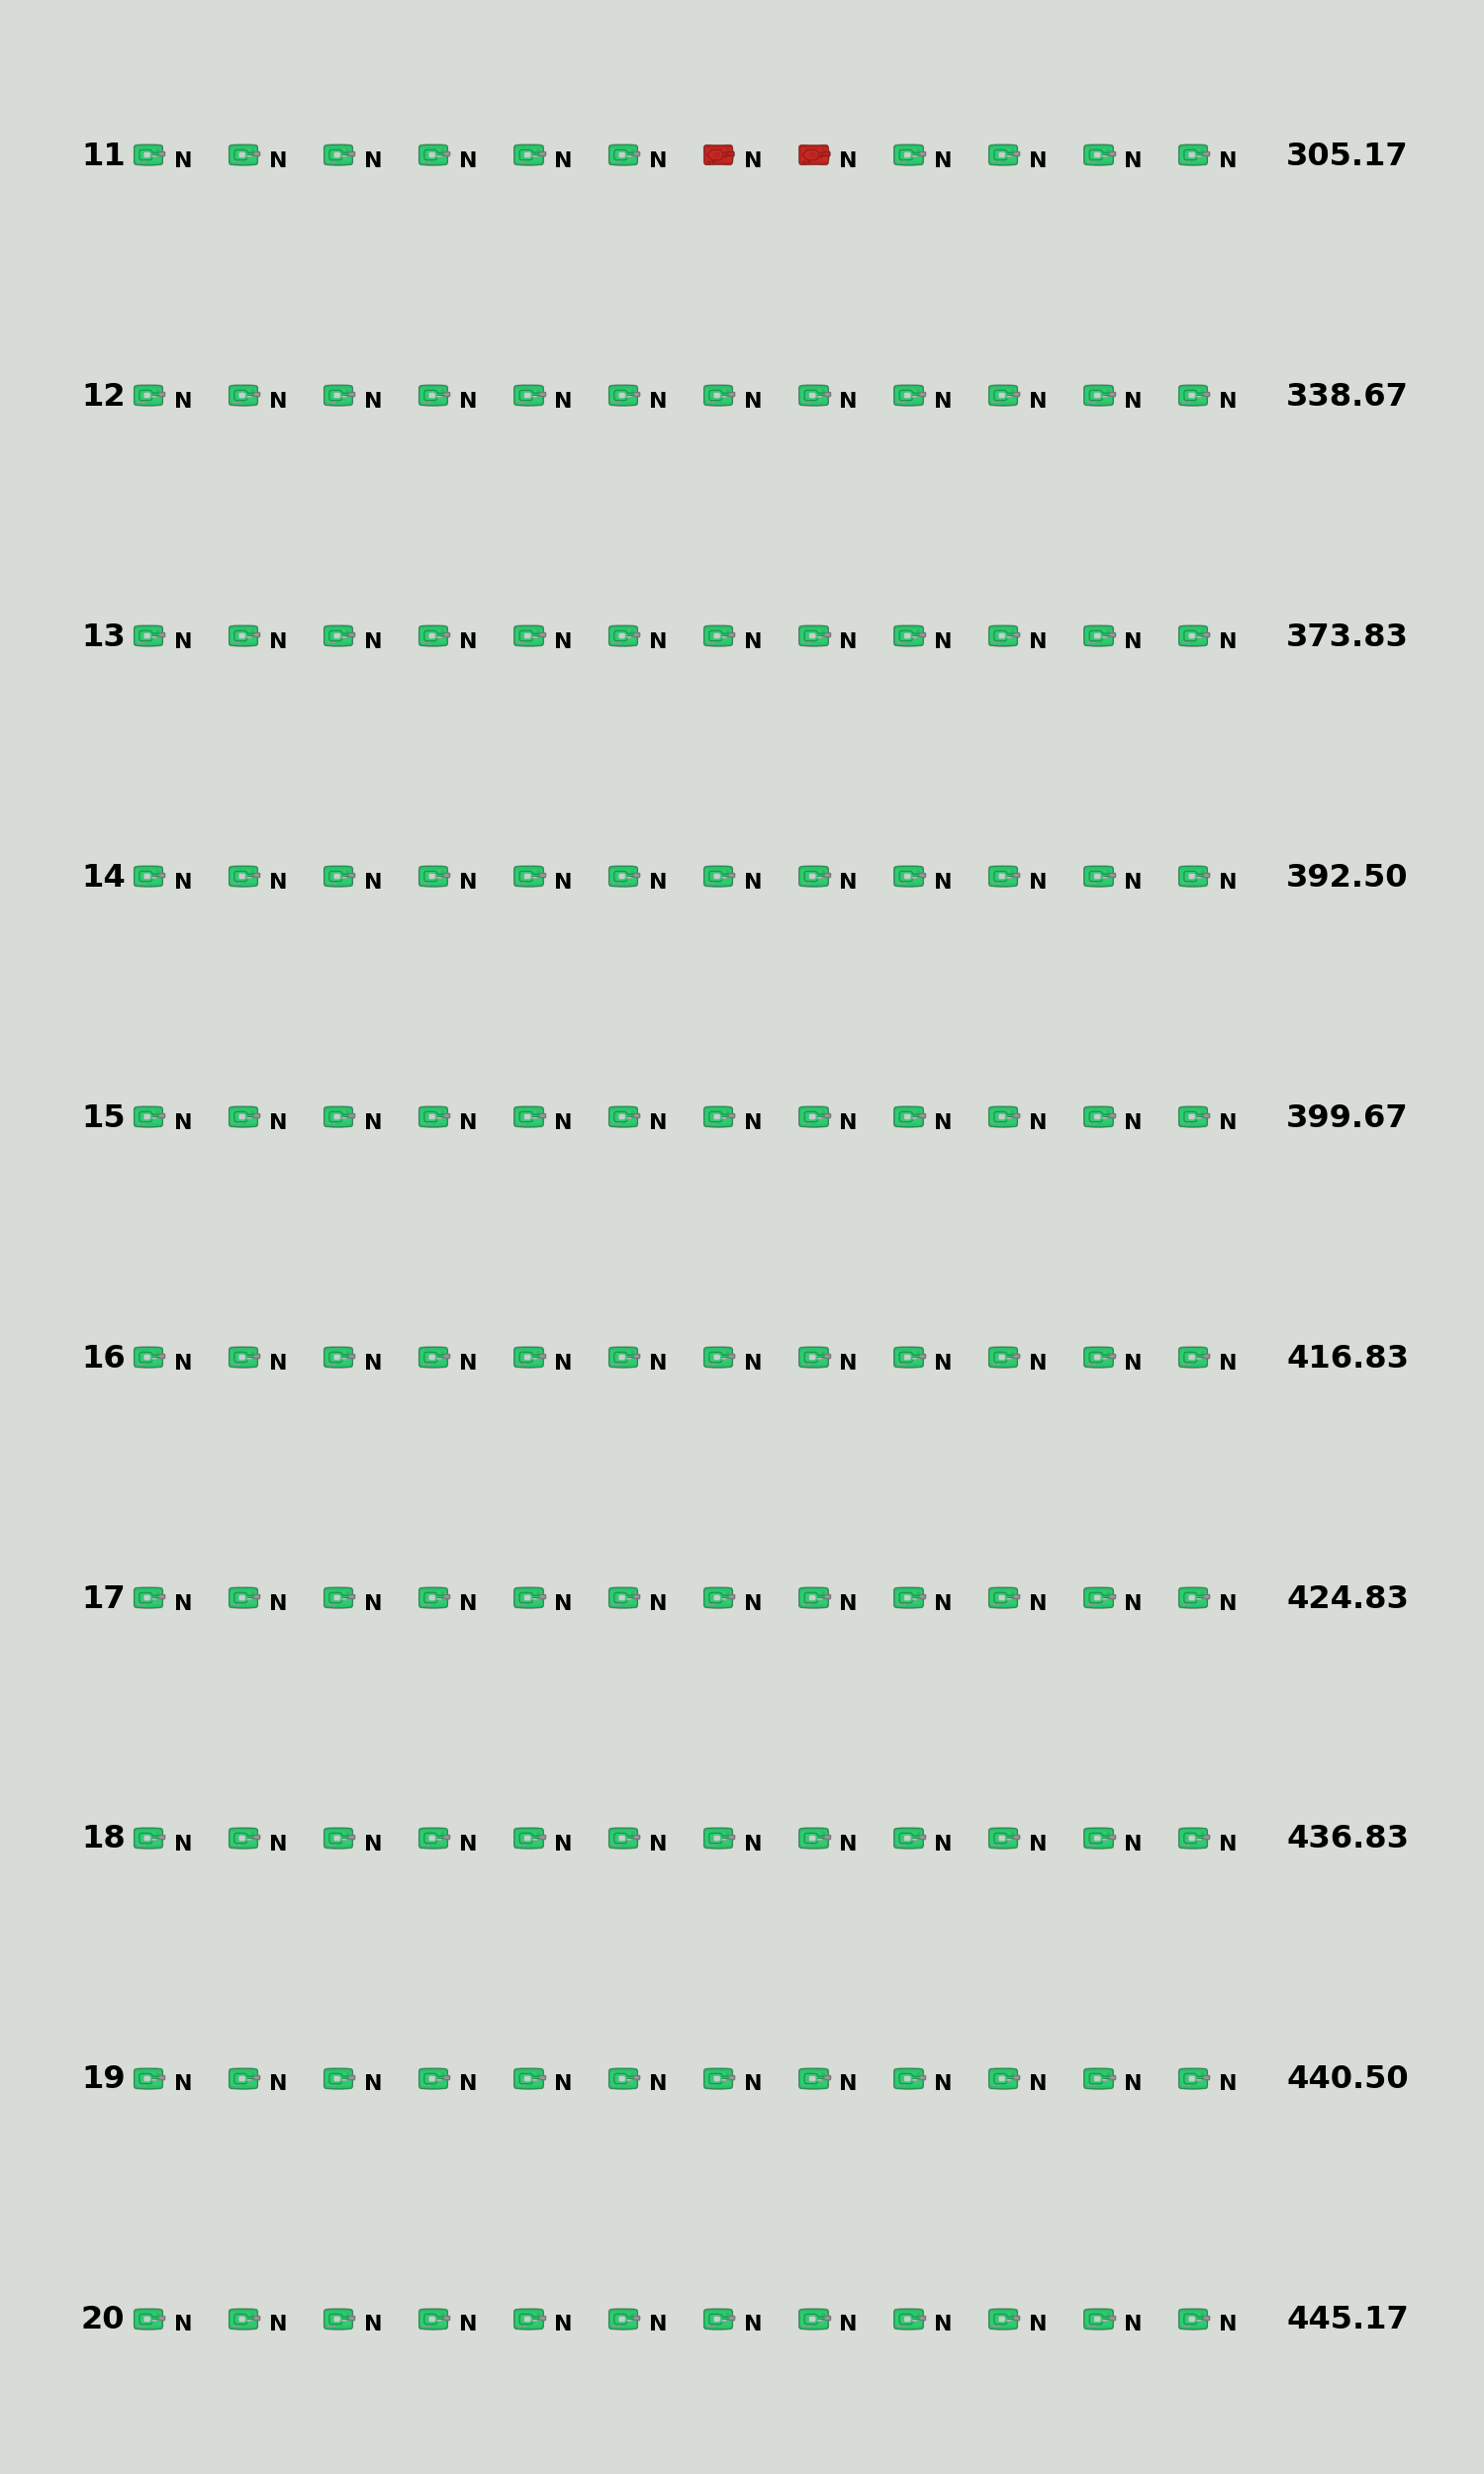
\includegraphics[width=0.9\textwidth]{figuras/td/td_redgreen_ai_mode_1_2.png}
  \caption{Visualização da moda de cada onda com a versão v1 contra Torres Vermelhas + Verdes.}
  \label{fig:td-moda-redgreen-1-2}
\end{figure}

\begin{figure}[H]
  \centering
  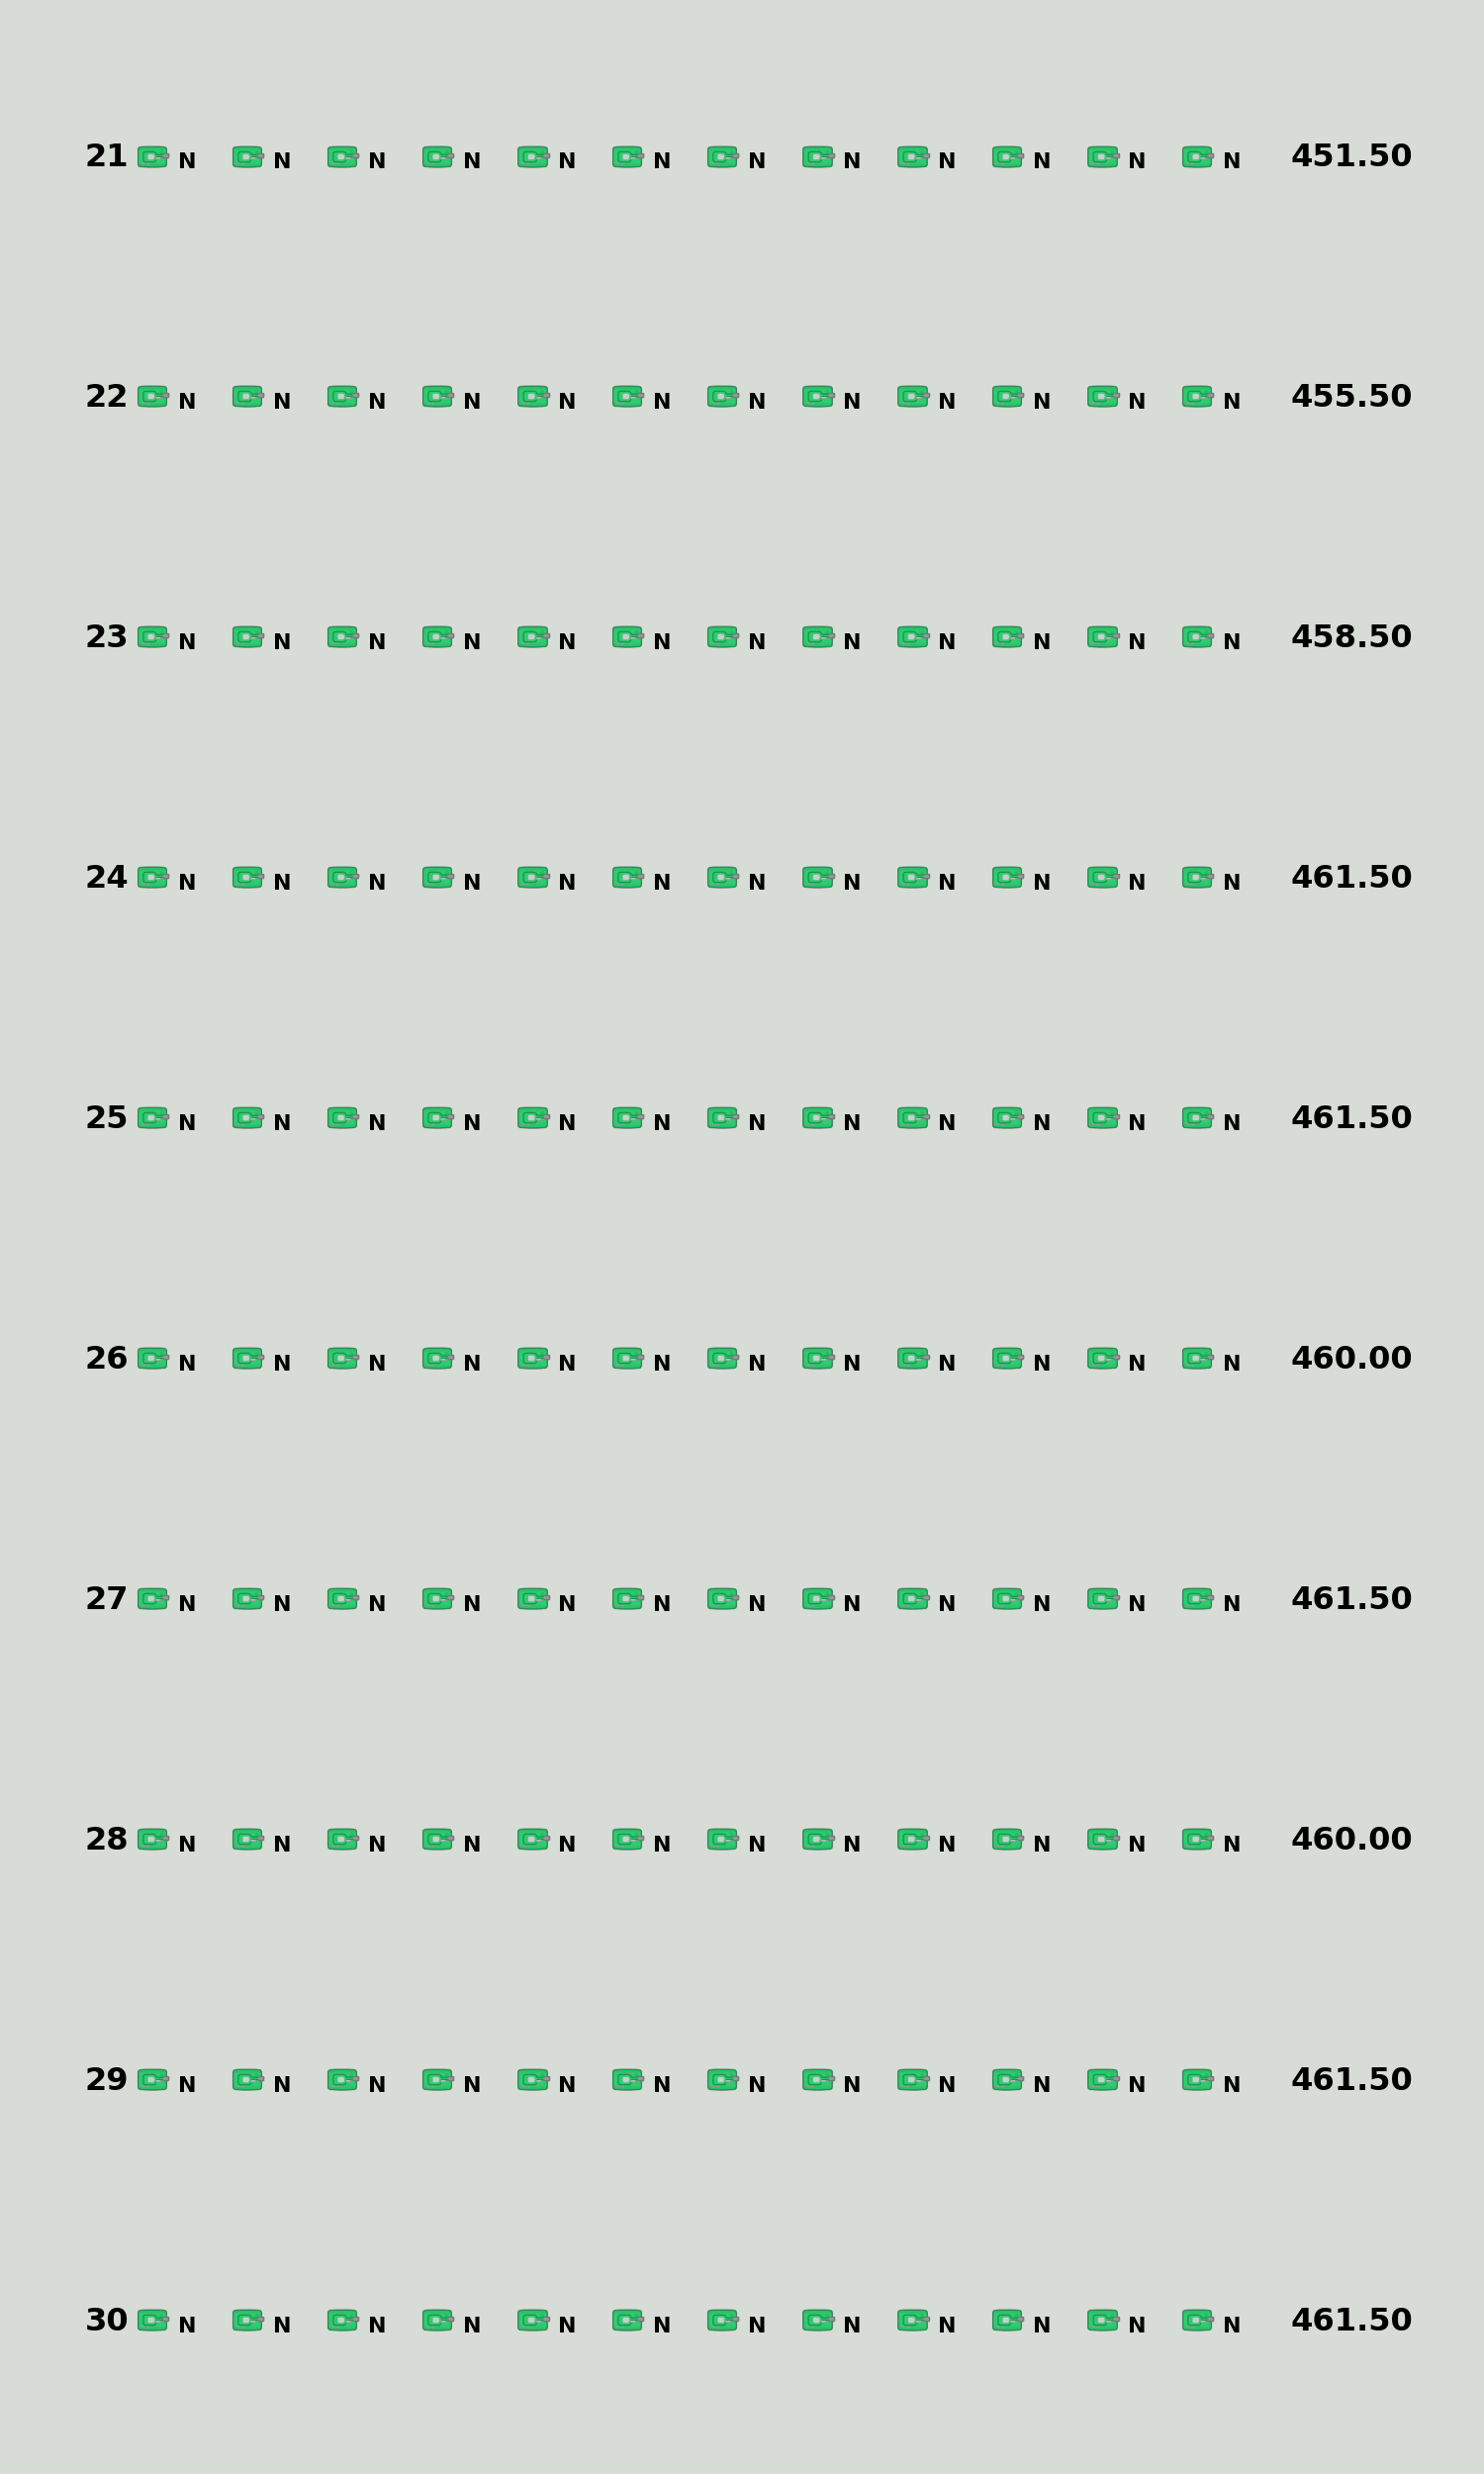
\includegraphics[width=0.9\textwidth]{figuras/td/td_redgreen_ai_mode_1_3.png}
  \caption{Visualização da moda de cada onda com a versão v1 contra Torres Vermelhas + Verdes.}
  \label{fig:td-moda-redgreen-1-3}
\end{figure}